

\section*{{Abstract:}}


	Suburbanization of poverty is a concerning trend in many urban regions. While research has described patterns of suburbanization of poverty at regional and neighbourhood levels, there are open questions about how lower-income households have agglomerated in the suburbs in recent history. Is suburban poverty primarily a result of 1) residential sorting within cities of low-income residents from central to suburban neighbourhoods (e.g. gentrification and displacement), 2) patterns of immigrant settlement in cities directed towards the suburbs, or 3) becoming and remaining poor while staying in the suburbs? The objective of this paper is to describe and quantify the propensity of these predominant individual geographic pathways of being poor and living in the suburbs. We do so via a cluster analysis of census and land-use data to define typologies of suburban neighbourhoods and then link this categorization to a large-scale panel dataset representing 20\% of tax filers in Canada (from 2006 to 2016). These data allow for analyzing how different pathways are observed within the context of large Canadian cities, specifically to what extent poverty in suburban neighbourhoods stems from intra-urban residential mobility, external immigration, and becoming poor in-place. We find that becoming poor while staying in the suburbs encompasses a greater proportion of suburban poverty than immigration and centre-to-suburb residential mobility combined. Overall, this research provides insight into the changing structure of urban neighbourhoods while also providing pertinent information to aid preventative policy aimed at reducing suburban poverty in Canada.
	


\section*{{Keywords:}}

suburbs, poverty, residential mobility, immigration, panel data



\section{Introduction}

Many urban regions have witnessed inner-city gentrification and growing concentrations of poverty in the suburbs over the past several decades \cite{ehrenhalt_great_2012,ades_are_2012,grant_changing_2020}. These trends have led to concerns of polarization and segregation of urban space by class and income \cite{hulchanski_three_2010}, negative impacts caused by gentrification and displacement on individual well-being \cite{elliott-cooper_moving_2020}, low quality of low-income housing in the suburbs \cite{august_gentrification_2018}, and reduced accessibility \cite{allen_planning_2020}, which can further compound poverty in suburban areas \cite{lucas_transport_2012}.

Ample research has described trends of suburbanization of poverty at regional and neighbourhood levels, for example by mapping neighbourhood changes in income or poverty rates, and showing how poverty is increasing in some suburban areas \cite{hulchanski_three_2010,ades_are_2012,breau_pulling_2018,grant_changing_2020}. However, neighbourhood-level analyses are limited in understanding how lower-income households have concentrated in more peripheral auto-oriented environments in recent history. Growth in poverty in neighbourhoods with suburban built environments could mainly be due to 1) residential sorting within cities of low-income residents from central to suburban neighbourhoods (e.g. gentrification and displacement), 2) patterns of immigrant settlement in cities directed towards the suburbs, or 3) becoming and remaining poor while living in the suburbs.  Understanding the propensity of these pathways can provide important knowledge regarding the urban dynamics that lead to contemporary suburban geographies of poverty concentration. Such knowledge can also be helpful for planning and policy including (but not limited to) public transit prioritization, providing resources for recent immigrants, protections against displacement, and social housing policy; and overall, aiming to reduce the burdens of being poor and living in the suburbs.

The objective of this paper is to document the predominant geographic pathways of becoming poor and living in the suburbs in Canada. We first provide a background and conceptual framework of different individual geographic pathways leading to suburban poverty. We then conduct an empirical analysis of census tract-level land-use data linked with an individual panel dataset pertaining to 20\% of Canadian tax filers to quantify the extent of different pathways to suburban poverty from 2006 to 2016 in the nine largest Census Metropolitan Areas (CMAs) in Canada. 
% Specifically, we use a combination of census and transportation network data to create a typology of suburbanization via a hierarchical $k$-means cluster analysis. We then link this typology to panel data representing 20\% of tax filers across Canada to examine immigrant settlement patterns and residential mobility trajectories of low-income households, grouped by typologies of suburbanization. 
Our analysis allows us to estimate to what extent suburban poverty stems from intra-urban residential mobility, external immigration, and remaining poor in-place---thus providing an important link between theory and empirical evidence on the urban dynamics that lead to suburbanization of poverty.


% 1) There is an increase in demand for inner-city living, specifically for housing in areas with high levels of accessibility. These rising costs could be driving lower-income households to move from central to suburban areas due to affordability issues i.e. due to gentrification and displacement \cite{freeman_displacement_2005,zuk_gentrification_2018}. 2) Similarly, suburban poverty could be forming due to spatial patterns of immigration. Recent immigrants often settle in the most affordable parts of cities, which due to the geograpahy of housing markets in many regions, are located in the suburbs \cite{bourne_changing_2001,bauder_residential_2002}. 3) Becoming and remaining poor within the suburbs. Low-income suburban areas could be forming due to compounding factors of poverty in place (such as social and transport disadvantage) limiting people's ability to access opportunities (e.g. jobs, education) needed for poverty reduction \cite{lucas_transport_2012,wilson_truly_2012}.


% We find that while the overall poverty rate has declined over time in Canadian cities, the total amount and relative rate of poverty in the suburbs has increased during this period. ... (more key findings here)

% This provides insight into the changing structure of urban environments as well as provide pertinent information to aid preventative policy aimed at reducing suburban poverty.

% \newpage


\section{Background}

% 1) background - what are the characteristics of suburbs, very brief history
% theory ? urban re-structuring

%From an economic perspective, the social and physical patterns of urban spatial structure can be considered as a result of competition for desirable space (demand), available land and property (supply), and the development of transportation technologies and networks \cite{alonso_location_1964,anas_urban_1998,glaeser_sprawl_2004}. 
% Early theories of urban growth saw this as combinations of aggregations of urban populations and expansion of urbanized land (i.e. expansion and intensification, concentration and de-centralization), that manifested itself in decreasing density and increasing wealth as one moves away from the city centre \cite{burgess_growth_1925}. People were seen to move up the social hierarchy by moving out away from the city via processes of succession and filtering, while the inner-city was the locus for in-migration and the working class \cite{burgess_growth_1925}. In the late 19th and early 20th century of early-industrializing nations, factories and industry tended to locate in the city centres, near major transport hubs. This lead to urban migration, people locating near the employment offered by such industry. However, these facilities also worsened the livability of central cities because of their noise and pollution, and the wealthy tended to live at further distances from the city centre, but still within commuting distance. During the 20th century, the private car, combined with auto-oriented planning and development led to expansive lower density built environments that were home to many middle- and upper-income households \cite{glaeser_sprawl_2004, baum-snow_did_2007,harris_creeping_2020}. 

% Today, many suburbs consist of dispersed detached dwellings centred around the car for daily mobility.

% The private car is often seen as a catalyst that took these ongoing trends, and put them into overdrive. The benefits of having a car were clear, it increased people's mobility and accessibility. They could travel to destinations more quickly, it increased the number of possible destinations that could be reached in a reasonable travel time, and it also increased the distances people were able to live to daily activity destinations. Indeed, many scholars have discussed theoretically, as well as shown empirically, that cars were a major driver of low-density auto-oriented suburban development during the 20th century \cite{glaeser_sprawl_2004, baum-snow_did_2007}. 
% aided by CMHC, etc. policy in the 20th century? - see Harris chapter

% HARRIS copied
% Government intervention also played a key role,
% encouraging mortgage indebtedness, amortization, and
% building and subdivision regulations to become the subur-
% ban norm.


% 2) urban restructuring - theory

Since the mid 20th century, many early-industrializing cities have witnessed a decline in middle-income jobs, increasing levels of wage and income inequality, and socio-spatial polarization. \cite{glaeser_inequality_2009,walks_income_2013,grant_changing_2020}. Many inner-city neighbourhoods have gentrified---i.e. once stagnating and declining urban neighbourhoods have undergone substantial investment and revitalization \cite{lees_gentrification_2013}. A result is that some lower-income households are being priced out of central parts of these cities, and are subsequently re-locating to less central, but more affordable neighbourhoods \cite{atkinson_measuring_2000,lees_gentrification_2013,zuk_gentrification_2018}. 

The reciprocal to inner-city gentrification is economic decline in suburbs \cite{ehrenhalt_great_2012}. Newer suburban housing stock in Canada remain predominately designed for middle- to upper-income households. However, lower-income residents are not primarily located in this typical suburban housing stock (e.g. single detached homes), but are often clustered in apartments in the suburbs \cite{skaburskis_filtering_2014,cooke_suburbanization_2015}. In Canada, these inner-suburban apartments include some social housing, but are mostly owned by private companies. These buildings are often noted at being at the bottom of the housing ladder due to their age (most were built during the mid-20th century), deterioration, and non-central locations \cite{skaburskis_filtering_2014, august_gentrification_2018}. Despite the presence of apartment towers, many of these neighbourhoods have built environments designed around the automobile, and have insufficient transit service \cite{allen_sizing_2019}. In major cities in Canada, the most affordable parts of cities are now found in the inner-suburbs, particularly in cities like Toronto and Vancouver where there has been substantial gentrification and increased demand for housing in older neighbourhoods near the core \cite{ades_are_2012,walks_income_2013,breau_pulling_2018,grant_changing_2020}. 




% 3) emp research sub poverty quick overview - should re-write this para to be different from prev paper

Research on suburbanization of poverty is typically based on longitudinal analysis of neighbourhood level census data, using this data to examine changes in the spatial distribution of low-income households or other socio-economic variables over time. Within the Canadian context, neighbourhood level studies have shown evidence of increasing intra- and inter-regional income inequalities \cite{bolton_growing_2012,chen_why_2012,walks_income_2013} and growing accounts of low-income residents concentrating in less central neighbourhoods, particularly in the inner-suburbs of Montreal, Toronto, and Vancouver \cite{ades_are_2012,pavlic_declining_2014,ades_is_2016,breau_pulling_2018, grant_changing_2020}. 

These existing studies on suburbanization of poverty focus on changes at a neighbourhood level (e.g. mapping the poverty level within neighbourhoods, and how this has changed over time). Neighbourhood level studies, while important for investigating patterns of regional socio-spatial restructuring, can suffer from ecological fallacies and are unable to directly examine individual pathways to suburban poverty. For example, inner-city gentrification and growing suburban poverty does not necessarily mean that low-income residents are being disproportionately displaced from central to suburban neighbourhoods. Observed neighbourhood changes might be due to upward mobility and downward mobility of residents who stay in these neighbourhoods. However, individual or household analyses addressing suburbanization of poverty are scarce relative to their neighbourhood-level counterparts, despite their importance in examining the causes and pathways to observed neighbourhood-level changes. This is mainly due to a lack of available panel-data with appropriate geographic precision, particularly for making population-level conclusions. Most neighbourhood change research uses publicly available census data, that due to privacy reasons, are pre-aggregated to spatial units (e.g. census tracts) \cite{logan_interpolating_2014,allen_new_2018}. These data are not available longitudinally at an individual level in most countries. 

There are a few studies that use other individual-level panel data sources to assess whether gentrification is linked to out mobility of low-income households, often framed in terms of displacement \cite{zuk_gentrification_2018}. In the United States, studies have made use of the Panel Study of Income Dynamics to examine residential mobility of low-income households. For example, studies using this data by \citeA{freeman_displacement_2005} and \citeA{delmelle_new_2020} have found that while low-income households are more likely to move than high income households overall, they are not more likely to move out of gentrifying areas \cite{freeman_displacement_2005} or from neighbourhoods proximate to newly opened transit lines \cite{delmelle_new_2020}. Other studies using panel data stemming from medical records in New York City \cite{dragan_does_2019} and tax records in Philadelphia \cite{ding_gentrification_2016} found similar results. Overall, recent reviews of literature summarizing whether, and to what extent, gentrification leads to displacement show mixed results and often focuses on specific case studies meaning that the topic remains open for debate \cite{rayle_investigating_2015,zuk_gentrification_2018, padeiro_transit-oriented_2019}. Furthermore, existing studies have also focused primarily on the neighbourhoods that are gentrifying and the in- and out-movers of these neighbourhoods, not the suburban neighbourhoods where poverty is increasing. In sum, it remains an open question as to what the predominant individual pathways to suburban poverty are. 


% concerns, problems
Despite these research gaps, regional trends of suburbanization of poverty have led to concerns pertaining to increased socio-spatial polarization of urban space \cite{hulchanski_three_2010,walks_income_2013,ades_are_2012}. Moreover, residential displacement can have substantial monetary costs, can upset social connections that are particularly important for impoverished households who rely on social support networks, and in some cases, can substantially negatively effect individual well-being  \cite{vigdor_does_2002,august_challenging_2014,elliott-cooper_moving_2020}. There are also concerns that some suburban apartment buildings have few on-site services and amenities, lack rent controls, and/or consist of decaying building structures \cite{short_decline_2007,august_gentrification_2018}. Living in suburban neighbourhoods can also quell the ability of low-income residents to travel to and participate in daily activities (e.g. travelling to work, shopping, accessing social services such as aid offices and non-profits that tend to concentrate in more central areas, and visiting friends and family), especially for those who are unable to afford a private vehicle \cite{allen_planning_2020}. Inability to access important destinations can result in social exclusion, which can also feedback and lead to prolonged poverty over time \cite{lucas_transport_2012}. However, it remains understudied how households end up to be poor and live in the suburbs. Research to date has primarily focused on neighbourhoods, rather than individuals. Yet our research is needed in order to further understand processes of urban dynamics leading to suburban poverty.





\section{Conceptual Framework}

In this section, we outline a conceptual framework describing potential geographic pathways to suburban poverty. These are grouped into three theoretical pathways. The first is based on internal residential sorting of low-income households from central to suburban areas, the second on external migration, and the third relates to remaining or becoming poor while staying in the suburbs. These are summarized below.



\textit{1) Centre-to-suburb residential mobility}

There are many causes of intra-regional migration and residential mobility. These are typically considered as a combination of demographic and household stage-of-life, household income, neighbourhood preferences, and the geography of housing supply and demand \cite{lee_neighborhood_1994,morrow-jones_housing_2005,schwanen_what_2005}. Low-income residential mobility is often framed in terms of displacement \cite{atkinson_measuring_2000,freeman_displacement_2005,zuk_gentrification_2018}. Displacement can pertain to forced causes like eviction, condo conversions, or building condemnation; or it can pertain to passive effects persuading residents to move, such as rent increases, deterioration in housing quality, or neighbourhood decline and loss of community connections \cite{zuk_gentrification_2018}. These factors are often discussed in the context of gentrifying neighbourhoods. Moving can be spurred by the broader forces of land markets and housing prices combined with household and stage-of-life factors. For example, a lower-income couple living in a gentrifying neighbourhood who wish to have a child would likely want a larger living space. Historically, they may have been able to rent a larger dwelling in the same neighbourhood, but given the demand and competition for housing in the neighbourhood, they may now have to look at different neighbourhoods. Moving to the suburbs can also be due to pull factors like better access to green space, newer housing, quality of schools, proximity to suburban employment, or to be closer to friends and family \cite{lee_neighborhood_1994,kim_intrametropolitan_2011,spring_influence_2017}. Regardless of the specific reason(s) for moving out of a central neighbourhood, it can often result in moving into a more affordable suburban neighbourhood, and subsequently in some cases, loss of community and social capital \cite{august_challenging_2014} and increased barriers to access important activity destinations, especially for non-drivers \cite{allen_planning_2020}.





\textit{2) Immigrant settlement:}

Many cities in the developed world continue to grow because of immigration rather than high fertility rates. Reasons for immigration include (but are not limited to) moving for opportunity (e.g. such as employment), a greater chance at social mobility, family reunification, and to escape poverty and oppression from their initial states \cite{boyd_100_2000,hagen-zanker_why_2008}. Urban immigrants can be classified as internal or international. While there are a number of moderate- to high-income immigrants, the majority of international immigrants enter Canadian cities at relatively lower levels of socio-economic status, on average, compared to existing residents, and are thus likely to settle where housing is more affordable \cite{kazemipur_invisible_2000}. As previously mentioned, the locations in many cities with the greatest abundance of more affordable housing are the inner-suburbs. Several studies have highlighted how Canadian suburbs are increasingly home to diverse immigrant communities \cite{bourne_are_1989,bourne_changing_2001,grant_changing_2020}. As well, immigrants often self-select into areas that already have a higher concentration of similar ethnicity. This can be due to social networks or direct family connections and access to social support services (e.g. specific language classes) as well as other neighbourhood amenities, such as access to specific grocery stores \cite{zhuang_role_2017,farber_transportation_2018}. Overall, these factors can lead to agglomerations of lower-income immigrant communities in the suburbs.
% Important to note is that interrants are also often excluded from auto mobility, at least upon arrival, often because of the costs of driving and time to get a driver's license, increasing their propensity to experiencing barriers to daily travel and activity participation \cite{clark_automobile_2010,lo_relationship_2011,farber_transportation_2018}.



\textit{3) Persistence of poverty in the suburbs:}

% NEED TO ADD MORE ABOUT NON-TRANSPORT/ACCESS FACTORS

% Concentration of poverty can have further feedback effects, such as increase in crime and urban decay, barriers to social mobility (e.g. Chetty, Hendren, & Katz, 2016), and limited resources due to a declining tax-base (Wilson, 2012). Jobs and other resources also became harder to obtain because of greater spatial distances. This has been termed as a ”buffer” effect (Wilson, 2012) or as spatial mismatch (Holzer, 1991), which is when the movement of people and firms from central city areas to the suburbs causes growing employment problems for people who live in inner-cities (especially, low income, and in the US, black residents).

Residents can also become and remain poor within the suburbs. Research on poverty in-place has pointed to causes relating to exposures to crime and urban decay, broader economic affects (such as the global financial crisis of 2007–2008), lack of collective efficacy and social capital, as well as inaccessibility to various social resources that can help alleviate poverty (e.g. employment, quality education, health care, social services, etc.). Many of these factors can interact and result in feedback effects, leading to prolonged poverty in certain locales \cite{wilson_truly_2012,sampson_great_2012}. Problems of inaccessibility, in particular, can be augmented by suburban built environments, which have predominantly been designed such that they necessitate having a car to enable societal participation \cite{urry_systemautomobility_2004,farber_my_2009,farber_running_2011}. Suburban built environments can deter active travel like walking or cycling often due to a lack of pedestrian and cycling infrastructure as well as dispersion of activity destinations \cite{ewing_travel_2010}. Public transit service is also often insufficient in many suburban auto-oriented environments. Overall, accessibility in the suburbs is greatly limited for those without cars. Car ownership has substantial costs for low-income households (e.g. due to up-front costs, loan payments, fuel, insurance, etc.) that are either not tenable, or result in increased financial stress since auto costs will usually make up a greater percent of their total income and limit spending in others domains \cite{klein_car_2017,walks_driving_2018, mattioli_vulnerability_2018}. If a household cannot afford access to a car, it can create barrier to daily travel and activity participation \cite{allen_planning_2020}. This can further increase risks of social exclusion and poverty as it can lead to inabilities in accessing employment opportunities, education, healthcare, and other social services \cite{lucas_transport_2012}. 

Continued poverty in suburban locations can also be further sub-divided into whether a resident stays in the same dwelling and neighbourhood, or if they move to different locations within the suburbs. Residential mobility of low-income suburban residents can be caused by the same displacement effects noted in 1), such as forced eviction or increasing rents \cite{august_gentrification_2018}, or it can be out of choice, such as wanting to change housing type due to stage of life factors or to move closer to work to reduce commute times \cite{morrow-jones_housing_2005}. Intra-suburban residential mobility can thus also have positive or negative effects on well-being and poverty alleviation, depending on the context.

Broad categories of transitions to suburban poverty are displayed in Figure \ref{path} via the prominent red lines. Growth of suburban poverty can thus be conceptualized as a combination of urban dynamics of housing markets and land use as well as preferences leading to 1) residential sorting within cities of low-income residents from central to suburban neighbourhoods, 2) patterns of immigrant settlement in cities directed towards the suburbs, or 3) becoming or remaining poor in the suburbs. The nodes \textit{centre} and \textit{suburb} on the graphic can also be interpreted as proxies for transport (dis)advantage. (It should be noted that this is a simple dichotomy, and could certainly be expanded to account for more than two discrete types of urban form). The following empirical research in this paper sets out to uncover the extent of these different pathways across Canadian cities and how they have changed over time.



\begin{figure}[h]
	\setlength{\fboxsep}{0pt}%
	\setlength{\fboxrule}{0pt}%
	\begin{center}
		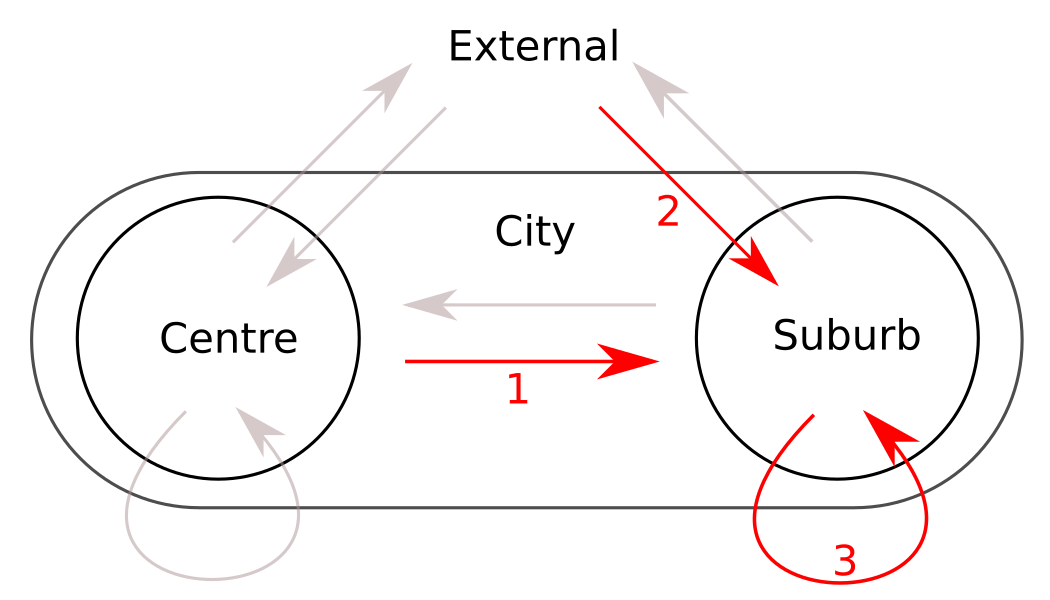
\includegraphics[width=3in]{figures/pathways.png}
		\caption{Theoretical individual geographic pathways to suburban poverty}
		\label{path}
	\end{center}
\end{figure}




\section{Data \& Methods}

Our methodology consists of several steps. First we use census and land use data to cluster neighbourhoods, specifically categorizing whether or not they are suburban (see Section 4.1). Second, we link this suburb-centre typology to an individual-level panel dataset of tax filers across Canada. Once we have this linked data, we describe overall trends of suburbanization of poverty by region (see Section 4.2). We then use this linked data to quantify the propensity of different pathways to suburban poverty described in our conceptual framework. Specifically for this analysis, we tabulate among residents in suburban poverty, the proportions of whom were living in different locations a year prior (e.g. what percent moved from a central neighbourhood, what percent immigrated in the past year, etc.), and examine how these proportions vary by CMA and how they change over time (see Section 4.3). In sum, our results provide new evidence of suburbanization of poverty in Canadian cities and how it is being formed.

Our analysis examines the nine largest Census Metropolitan Areas (CMA) in Canada. CMAs are agglomerations of municipalities where at least 50\% of the employed labour force works in the region's core \cite{statistics_canada_dictionary_2016-1}. While not perfect definitions of what consist of an urban area, CMAs are commonly used as study areas for urban research in Canada, and have been specifically used to examine neighbourhood change \cite{walks_income_2013,grant_changing_2020} and suburbanization of poverty \cite{ades_are_2012,allen_suburbanization_2021}. In descending order of their population in 2016, the nine CMAs for this study are Toronto, Montréal, Vancouver, Calgary, Edmonton, Ottawa-Gatineau, Winnipeg, Québec, and Hamilton. Each of these CMAs had a population of greater than 700,000 in 2016, while all other CMAs in Canada had a population of less than 600,000. In 2016, these nine CMAs accounted for 55\% of Canada's population.



% could do a line plot of popultion over time?

% para on their prev research of neigh change in these cities

%In  Canada,  there  is  evidence  of  increasing  income  inequalities  both  within  and  between  re-gions  (Walks,  2013;  Bolton  &  Breau,  2012;  Breau,  2015;  Chen,  Myles,  &  Picot,  2012),  as  wellas concentrations of low-income households forming in some inner-suburban neighborhoods(Ades  et  al.,  2012;  Pavlic  &  Qian,  2014;  Ades  et  al.,  2016;  Breau  et  al.,  2018).   For  example,Pavlic and Qian (2014) classified census tracts by density, age of housing stock, and distance todowntown and found that there has been decline or stagnation in prosperity in inner-suburbanareas relative to central areas and newer outer-ring suburbs. Research by Ross et al. (2004) andAdes et al. (2012) computed spatial segregation indices on low-income households and house-holds in poverty in Canadian cities, each finding that economic segregation is increasing at aneighborhood level and that low-income households are becoming increasingly concentratedand isolated within cities’ spatial units. Statistical mapping exercises have also highlighted thatneighborhoods with higher concentrations of low-income households are located further fromthe downtown core over the past several decades (Ades et al., 2012; Breau et al., 2018).


% rough description, e.g. Cg and Ed a bit newer, 

% Age of their development. Calgary and Edmonton, for example, have undergone the vast majority of their growth since World War Two, QQQ suburban compared to eastern cities. - move to results?



\subsection{Classifying Suburbs}

Our analysis begins by classifying neighbourhoods based on their urban form via a cluster analysis. The main objective of this analysis is to encode the suburban status of different neighbourhoods in order to subsequently link to data on residential mobility.

Creating classifications of neighbourhoods has a long history \cite{booth_life_1902,shevky_social_1955} and there is currently a rich literature on generating typologies of neighbourhoods via quantitative cluster analysis techniques  \cite{delmelle_differentiating_2017,silver_markov_2021}. However, most existing research has focused on clustering based on demographic and socio-economic characteristics (often framed in terms of geodemographics or market segmentation). Fewer studies have used clustering on urban form variables to try to specifically characterize whether or not a neighbourhood is suburban. Previous research that has attempted to identify suburban neighbourhoods within a city have instead adopted threshold approaches that define suburbs based on whether a neighbourhood has certain attributes above or below specific thresholds (e.g. if the population density is less than $\theta$) \cite{moos_suburban_2015,airgood-obrycki_suburban_2019}. While simple to interpret, these approaches are limited by their arbitrary selection of thresholds (e.g. the selection $\theta$). 

% Other previous research has also adopted creating numeric indices of sprawl-compactness, based on dimensionality reduction techniques like factor analysis \cite{ewing2014measuring}. However, such indices are limited in terms of discerning qualitative differences among neighbourhoods with similar scores as well as inability to assess hierarchical grouping of neighbourhoods. 

To generate classifications of Canadian suburbs, we adopt a combined hierarchical $k$-means approach. Similar approaches have been used in studies generating socio-economic typologies of neighbourhoods in Toronto \cite{silver_markov_2021} and across the United Kingdom \cite{vickers_creating_2005} to limit the drawbacks of solely using hierarchical or partitional methods (e.g. such as the random selection of cluster centres in $k$-means).
% Importantly, for our analysis, this approach allows us to initially differentiate between suburbs and central neighbourhoods (as in our conceptual framework shown in Figure \ref{path}), and it further allows us to examine different groups of suburban neighbourhoods. 
Specifically, the hierarchical $k$-means method is a three step process; it first uses hierarchical clustering to cut the tree into $k$-clusters, then it computes the means of each cluster, and third it uses $k$-means to group observations based on these cluster means. For our study, we initially aim to generate two clusters, \textit{centre} and \textit{suburb}, in order to subsequently examine pathways to poverty in the suburbs. However, our approach could be extended to generate sub-groups of each (this is noted as a direction for future work in the concluding section of this paper).

We use Census Tracts (CT) as spatial representations of neighbourhoods, because of data availability and because they are the most common spatial unit used in neighbourhood change studies in Canadian cities \cite{allen_new_2018,grant_changing_2020}. CTs usually have a population between 2,500 and 8,000 residents. Variables inputted into our cluster analysis are described below. These variables were selected based on their use in previous studies to measure how suburbanized a neighbourhood is, each capturing an important dimension of suburbanization, as well as data availability for Canadian CMAs at the CT level.

\begin{itemize}
	\item \textit{Population density.} Suburbs are often characterized as having lower densities than central neighbourhoods \cite{torrens2000measuring,hanibuchi_does_2012, massey_suburbanization_2018,airgood-obrycki_suburban_2019}. We thus use population density based on data from the 2016 Canadian census as an input into our cluster analysis.
	
	\item \textit{Age of housing}. While the history of suburbs in North America date back to before the 20th century, the sprawling scale and hyper-automobile focused design of suburbs expanded greatly after World War Two \cite{airgood-obrycki_suburban_2019,harris_creeping_2020}. Similar to previous studies measuring suburbanization \cite{hanibuchi_does_2012,ades_is_2016,airgood-obrycki_suburban_2019}, we also include a variable into our cluster analysis that pertains to age of housing, specifically the percentage of dwellings in a neighbourhood that were built after 1945.
	
	\item \textit{Type of housing}. Suburban housing is commonly characterized as being composed of single-detached dwellings 	\cite{moos_suburban_2015, ades_is_2016}. 
	% In Canadian cities, some suburban neighbourhoods also include semi-attached housing and apartment buildings. Particularly during the mid-20th century, there were a number of apartment buildings erected in the inner-suburbs. In the late 20th and early 21st centuries, there were also development of new urbanist neighbourhoods with a variety of housing types in peripheral suburban locations \cite{xu_is_2017}. 
	As such, we include a variable for the percent of dwellings in an neighbourhood that are single-detached.
	
	\item \textit{Regional accessibility}. Accessibility, within the context of urban and transportation geography, often refers to the ability to reach activity destinations in a reasonable amount of time \cite{hansen_how_1959,geurs_accessibility_2004}. (A very simple measure of regional accessibility is distance from a neighbourhood to the central business district). More detailed accessibility to jobs measures are often used as a proxy for regional accessibility, and have specifically previous been used to assess how centralized (or suburbanized) a neighbourhood is \cite{torrens2000measuring,zhang_dynamics_2020}. For our study, we make use of previously generated measures of transit accessibility to jobs that were designed to allow for comparison between regions by accounting for competition for employment and multi-modal transportation networks, including detailed transit schedules \cite{allen_measure_2020}. We use a transit accessibility measure, rather than an auto accessibility measure to additionally account for transit deficits in suburban areas. (However, it should be noted that transit accessibility and auto accessibility measures are quite correlated, with $r = 0.84$, so they would likely achieve similar results). The mathematical formulation and description of input datasets for the transit accessibility measure borrowed from \citeA{allen_measure_2020} are described in the Appendix.
	
	\item \textit{Local accessibility}. Local built environment and accessibility measures are often used to assess the effects of sprawl on health outcomes \cite{ewing_relationship_2003}, travel behaviour \cite{ewing_travel_2010}, and specifically to quantify how suburban a neighbourhood is \cite{ewing2014measuring}. For this study, we use the Proximity Measures Database (PMD) produced by Statistics Canada, which consists of walking distances to various amenities at the census dissemination block level \cite{statistics_canada_proximity_2020}. We sum the standard scores of walking access to eight types of destinations; pharmacies, childcare, healthcare, primary education, secondary education, libraries, parks, and grocery stores to create an overall metric of local amenity proximity and walkability. Details on each individual component are included in the Appendix.
	
\end{itemize}

Prior to clustering, CTs from all nine CMAs were combined into one dataset, and then all variables are normalized. This allows for direct comparison of results between cities, since all variables and results are based on the same scale. All input data were based on data circa 2016 when there were 3,947 CTs across all nine CMAs in total. However, 44 CTs were missing data in 2016, so they were not included in the cluster analysis, resulting in an $n = 3,903$. The omitted 44 CTs only accounted for 0.006\% of the overall population. 


\subsection{Measuring Suburbanization of Poverty}

Next we link this neighbourhood typology to longitudinal micro-data, specifically to the Longitudinal Administrative Database (LAD) \cite{government_of_canada_longitudinal_2020}. The LAD is a 20\% Bernoulli sample of tax filers across Canada. Sampling is completely random across Canada, so there is no non-random bias for any particular geographic area. The data consists of an annual panel, and includes a suite of information that residents note on their tax returns. In 2006, $n = 2,551,013$ in all nine CMAs combined, and in 2016, $n = 2,965,778$. The data include a vector of sampling weights, which we use for all of our analysis and presenting data as population totals. The data also denote births and are additionally linked with immigration records indicating whether, and if so when, residents immigrated into Canada. The LAD has primarily been used for research on examining usage of tax saving accounts \cite{berger_empirical_2019}, regional labour markets \cite{albouy_local_2019}, and income over the life course \cite{denton_age-income_2019}. Importantly, the LAD denote the six-digit postal code (which usually consist of a single apartment building or city block) as well as the CT of residence on December 31st for each tax year meaning they have great potential to also be used for research on residential mobility, and specifically for this paper, analyzing individual pathways to suburban poverty. Given the individual nature of the data, the data were accessed at Statistics Canada's secure Research Data Centre (RDC). Because of privacy concerns, any tabular data outputs from the RDC could only be exported as population-level weighted totals and individual cells of exported tabular data had to have a minimum of 100 unweighted observations.

The main variable of interest is the low-income status of tax filers. We use this variable as an indicator of household poverty. In the LAD, low-income status is pre-coded as a binary classification based on the Low-Income Measure (LIM). The LIM is a threshold defined by Statistics Canada whether the household has an income less than 50\% of the regional median adjusted household income---where adjusted pertains to dividing a household's income by the square root of the number of members in the household. This is to account for when a household increases in size, its needs increase, but at a decreasing rate. The LIM is provided as a before-tax and as an after-tax measure. We use the after-tax measure for our analysis. The LIM has previously been used to assess poverty in Canada among recent immigrants \cite{picot_immigration_2014}, in relation to transit accessibility \cite{allen_sizing_2019}, and analyzing food insecurity \cite{brown_money_2019}. 

For our study, linking this data to the results of the cluster analysis described in the previous section allows for describing the growth or decline of poverty in Canadian suburbs. We track this with three indices. The first is simply the total number of residents living below the poverty line in the \textit{suburbs}, $L_S$. This allows for understanding the overall scale of suburban poverty and how it has changed over time. Our next two indices are similar to the centralization indices described by \citeA{duncan_methodological_1955} and previously used in Canada with census data \cite{ades_are_2012}, but are re-focused on poverty concentration in the suburbs rather than the centre. Specifically, the second index we calculate is the percent of that population that is below the LIM threshold who live in the \textit{suburbs}, $L_S / (L_S + L_C)$, i.e. this is the probability of living in the \textit{suburbs} if living under the poverty line. However, this index is limited since it does not account for the overall population, or the growth or decline of such, in the \textit{suburbs} relative to the \textit{centre} (i.e. $L_S / (L_S + L_C)$ may be increasing mainly because the overall population in the suburbs, $N_S$, is increasing as well). As such, thirdly, we compute a relative measure to show whether poverty has suburbanized over time relative to the centre. This is the poverty rate in the \textit{suburbs} divided by the poverty rate in the \textit{centre}, $(L_S / N_S) / (L_C / N_C)$. An increase in this ratio indicates that poverty is suburbanaizing over time. This index is similar to the commonly used centralization index \cite{duncan_methodological_1955,massey_dimensions_1988}, but is based on the dichotomous results of our multivariate cluster analysis, rather than distance to the central business district.


% LAD data dictionary (2014) https://www23.statcan.gc.ca/imdb-bmdi/document/4107_D9_T15_V2-eng.pdf

% LAD more info https://crdcn.org/datasets/lad-longitudinal-administrative-databank





\subsection{Mobility Pathways to Suburban Poverty}

Importantly, this linked data allows for describing the individual geographic pathways to suburban poverty based on the conceptual framework outlined in Section 3. The data are annual panel data, meaning that individuals can be tracked over time. For our study, we are interested in whether and how residential locations changes over time, specifically in reference to those who are poor and living in the suburbs. 

We first quantify for each year, $t$, for different population groups, population counts pertaining to where they were living the year prior (i.e. in $t-1$). These counts are represented as $N_{i,j}$. For example, if $i$ is living in a city centre in year $t-1$, and $j$ is living in the suburbs in year $t$, then $N_{i,j}$ is the number of residents currently living in the suburbs ($j$) that lived in the city centre ($i$) the year prior. We have several categories of prior residential states ($i \in I$). For states 1-4, the data are further divided by low-income status.


% $P_{i|j}$ where $i$ and $j$ pertain to residential locations at time periods $t-1$ and $t$ respectively.   For our main analysis, proportions are held to $\sum_j P_{i|j} = 1$. 

\begin{enumerate}
	\item Same postal code (i.e. most likely did not move during the one-year time period).
	\item Moved from the \textit{centre} of their CMA (based on the cluster analysis results).
	\item Moved from a \textit{suburb} in their CMA (based on the cluster analysis results).
	\item Moved from elsewhere in Canada, but from outside their current CMA.
	\item Immigrated from another country.
	\item Persons born within the past year (included because the data represent entire populations)
\end{enumerate}

And we have four current residential states, $j \in J$, at time $t$, as follows. Our focus is on the transitions to low-income prevalence in the suburbs, while the other three serve as comparisons. 

\begin{enumerate}
	\item Low-income people living in a \textit{suburb}. 
	
	\item Low-income people living in the \textit{centre}
	
	\item Not low-income people living in a \textit{suburb}, 
	
	\item Not low-income people living in the \textit{centre}
\end{enumerate}

We use $N_{i,j}$ to then estimate the probability of coming from state $i$, given being in state $j$. In other words, this directly allows for showing among those in suburban poverty, the percent of which came from each of the different states, $i$. Similar statistics have been computed in residential mobility research tracking moves between different types of tenure \cite{withers_methodological_1997} and components of housing quality \cite{patel_effects_2020}. These are computed as follows:



\begin{equation}
P(i|j) = 100 \frac{N_{i,j}}{\sum_j N_{i,j}}
\end{equation}


The multiplication by 100 is to represent results as percents. We generate $P(i|j)$ and first summarize our results for the average proportions across a 10 year period (2006 to 2016). Second, we plot $P(i|j)$ for each pair of years in order to examine how these have changed over time. And third, we summarize for each CMA to highlight how different urban regions have varying propensities in their pathways to suburban poverty. 

Additionally we compute what the probability is of moving to state $j$, given previously being in state $i$. For example, this allows for showing, for different groups of people (e.g. international immigrants), what the probability is that they will end up in poverty and living in the suburbs in the following year. This is computed as follows:


\begin{equation}
P(j|i) = 100 \frac{N_{i,j}}{\sum_i N_{i,j}}
\end{equation}





\section{Results}

\subsection{Classifying Suburbs}

We first present the results of grouping neighbourhoods based on their urban form. The initial partition ($k = 2$) of our analysis classifies census tracts as \textit{suburb} and \textit{central} neighbourhoods. The means of the cluster input variables for these two groups are shown in Table \ref{table:k2}. Similar to previous research, we find that one of our groups (which we thus term as \textit{suburban}), neighbourhoods have a much lower population density \cite{hanibuchi_does_2012, massey_suburbanization_2018,airgood-obrycki_suburban_2019}, local accessibility \cite{ewing2014measuring}, and regional accessibility \cite{torrens2000measuring,zhang_dynamics_2020}, while having a much greater propensity of single-detached dwellings \cite{moos_suburban_2015, ades_is_2016}.


\begin{table}[h]
	\small
	\centering
	\caption{{Summary statistics (2016) of the partition of census tracts into two groups}}
	\label{table:k2}
	\begin{tabular}{lll}
		\hline
		& \textit{Centre}    & \textit{Suburb}   \\ \hline
		\textit{n} census tracts   & 994     & 2,909     \\
		Total population (1000s)         & 4,080   & 14,319 \\
		Mean population density (persons / km$^2$)        & 10,217   & 2,772     \\
		Mean detached dwellings         & 13.5\%   & 53.7\%    \\
		Mean post-1945 dwellings           &  75.1\%       &  97.1\%        \\
		Mean regional accessibility (Z) & 1.26    & -0.446   \\
		Mean local accessibility (Z)    & 1.23    & -0.428   \\
		\hline
	\end{tabular}
\end{table}

\begin{figure*}[h]
	\setlength{\fboxsep}{0pt}%
	\setlength{\fboxrule}{0pt}%
	\begin{center}
		\centering
		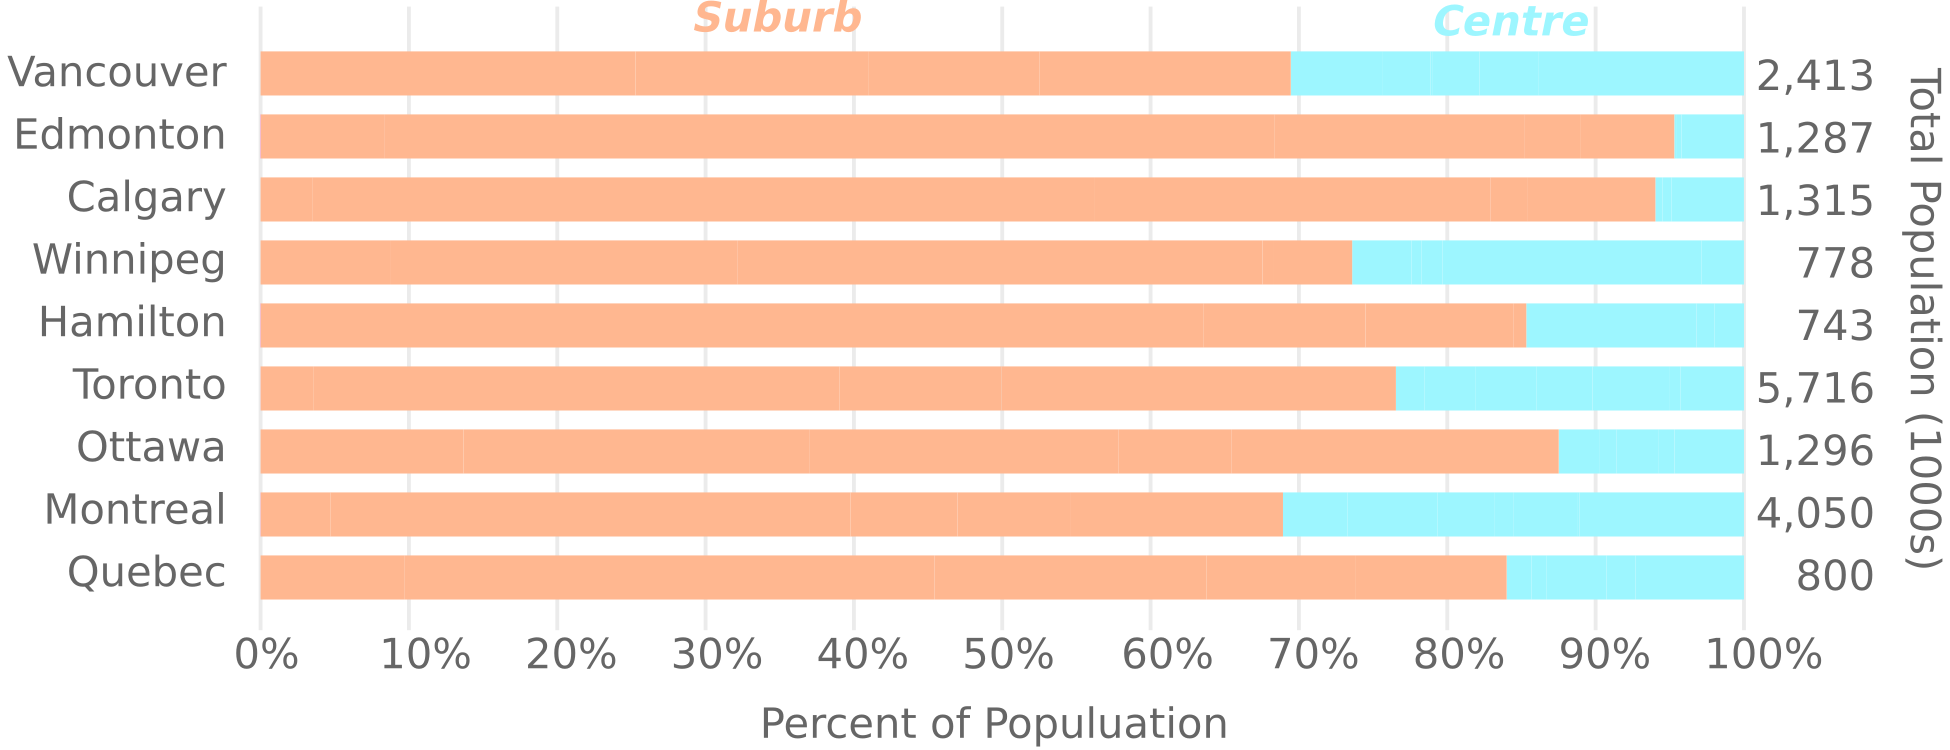
\includegraphics[width=5in]{figures/cluster_by_city.png}
	\end{center}
	\caption{Distribution of population for each cluster group by CMA}
	\label{kcma}
\end{figure*}



Census tracts from nine CMAs were inputted into the cluster analysis. However, because of the varying histories of growth and local policies as well as environmental constraints in each CMA, each has a different spatial distribution of urban form typologies, and importantly, different proportions of neighbourhoods that are classified as a \textit{suburb}. Figure \ref{kcma} displays the distribution of cluster groups in each CMA (maps of each CMA are included in the Appendix). For all CMAs, the majority of the population lives in suburban neighbourhoods. This is expected since the population of most of these CMAs has more than tripled since 1945, and the majority of urban development has been of a suburban form. Montreal and Vancouver have the lowest percent of their population living in suburban areas, with just under 70\%. In Montreal's case, this is mainly because it was the largest Canadian city during the 19th and early 20th century, and thus has the greatest extent of pre-auto-oriented development. For Vancouver, the relatively lower percent of suburbs is partly due to geographic constraints (mountains and the ocean) limiting sprawl. Conversely, in Calgary and Edmonton, approximately 95\% of the population lives in the suburbs. These two Albertan cities have few topographic constraints and the vast majority of their urban development has occurred during the auto-oriented post-war period.




% \newpage

%\begin{figure*}[h]
%	%	\setlength{\fboxsep}{0pt}%
%	%	\setlength{\fboxrule}{0pt}%
%	\begin{center}
%		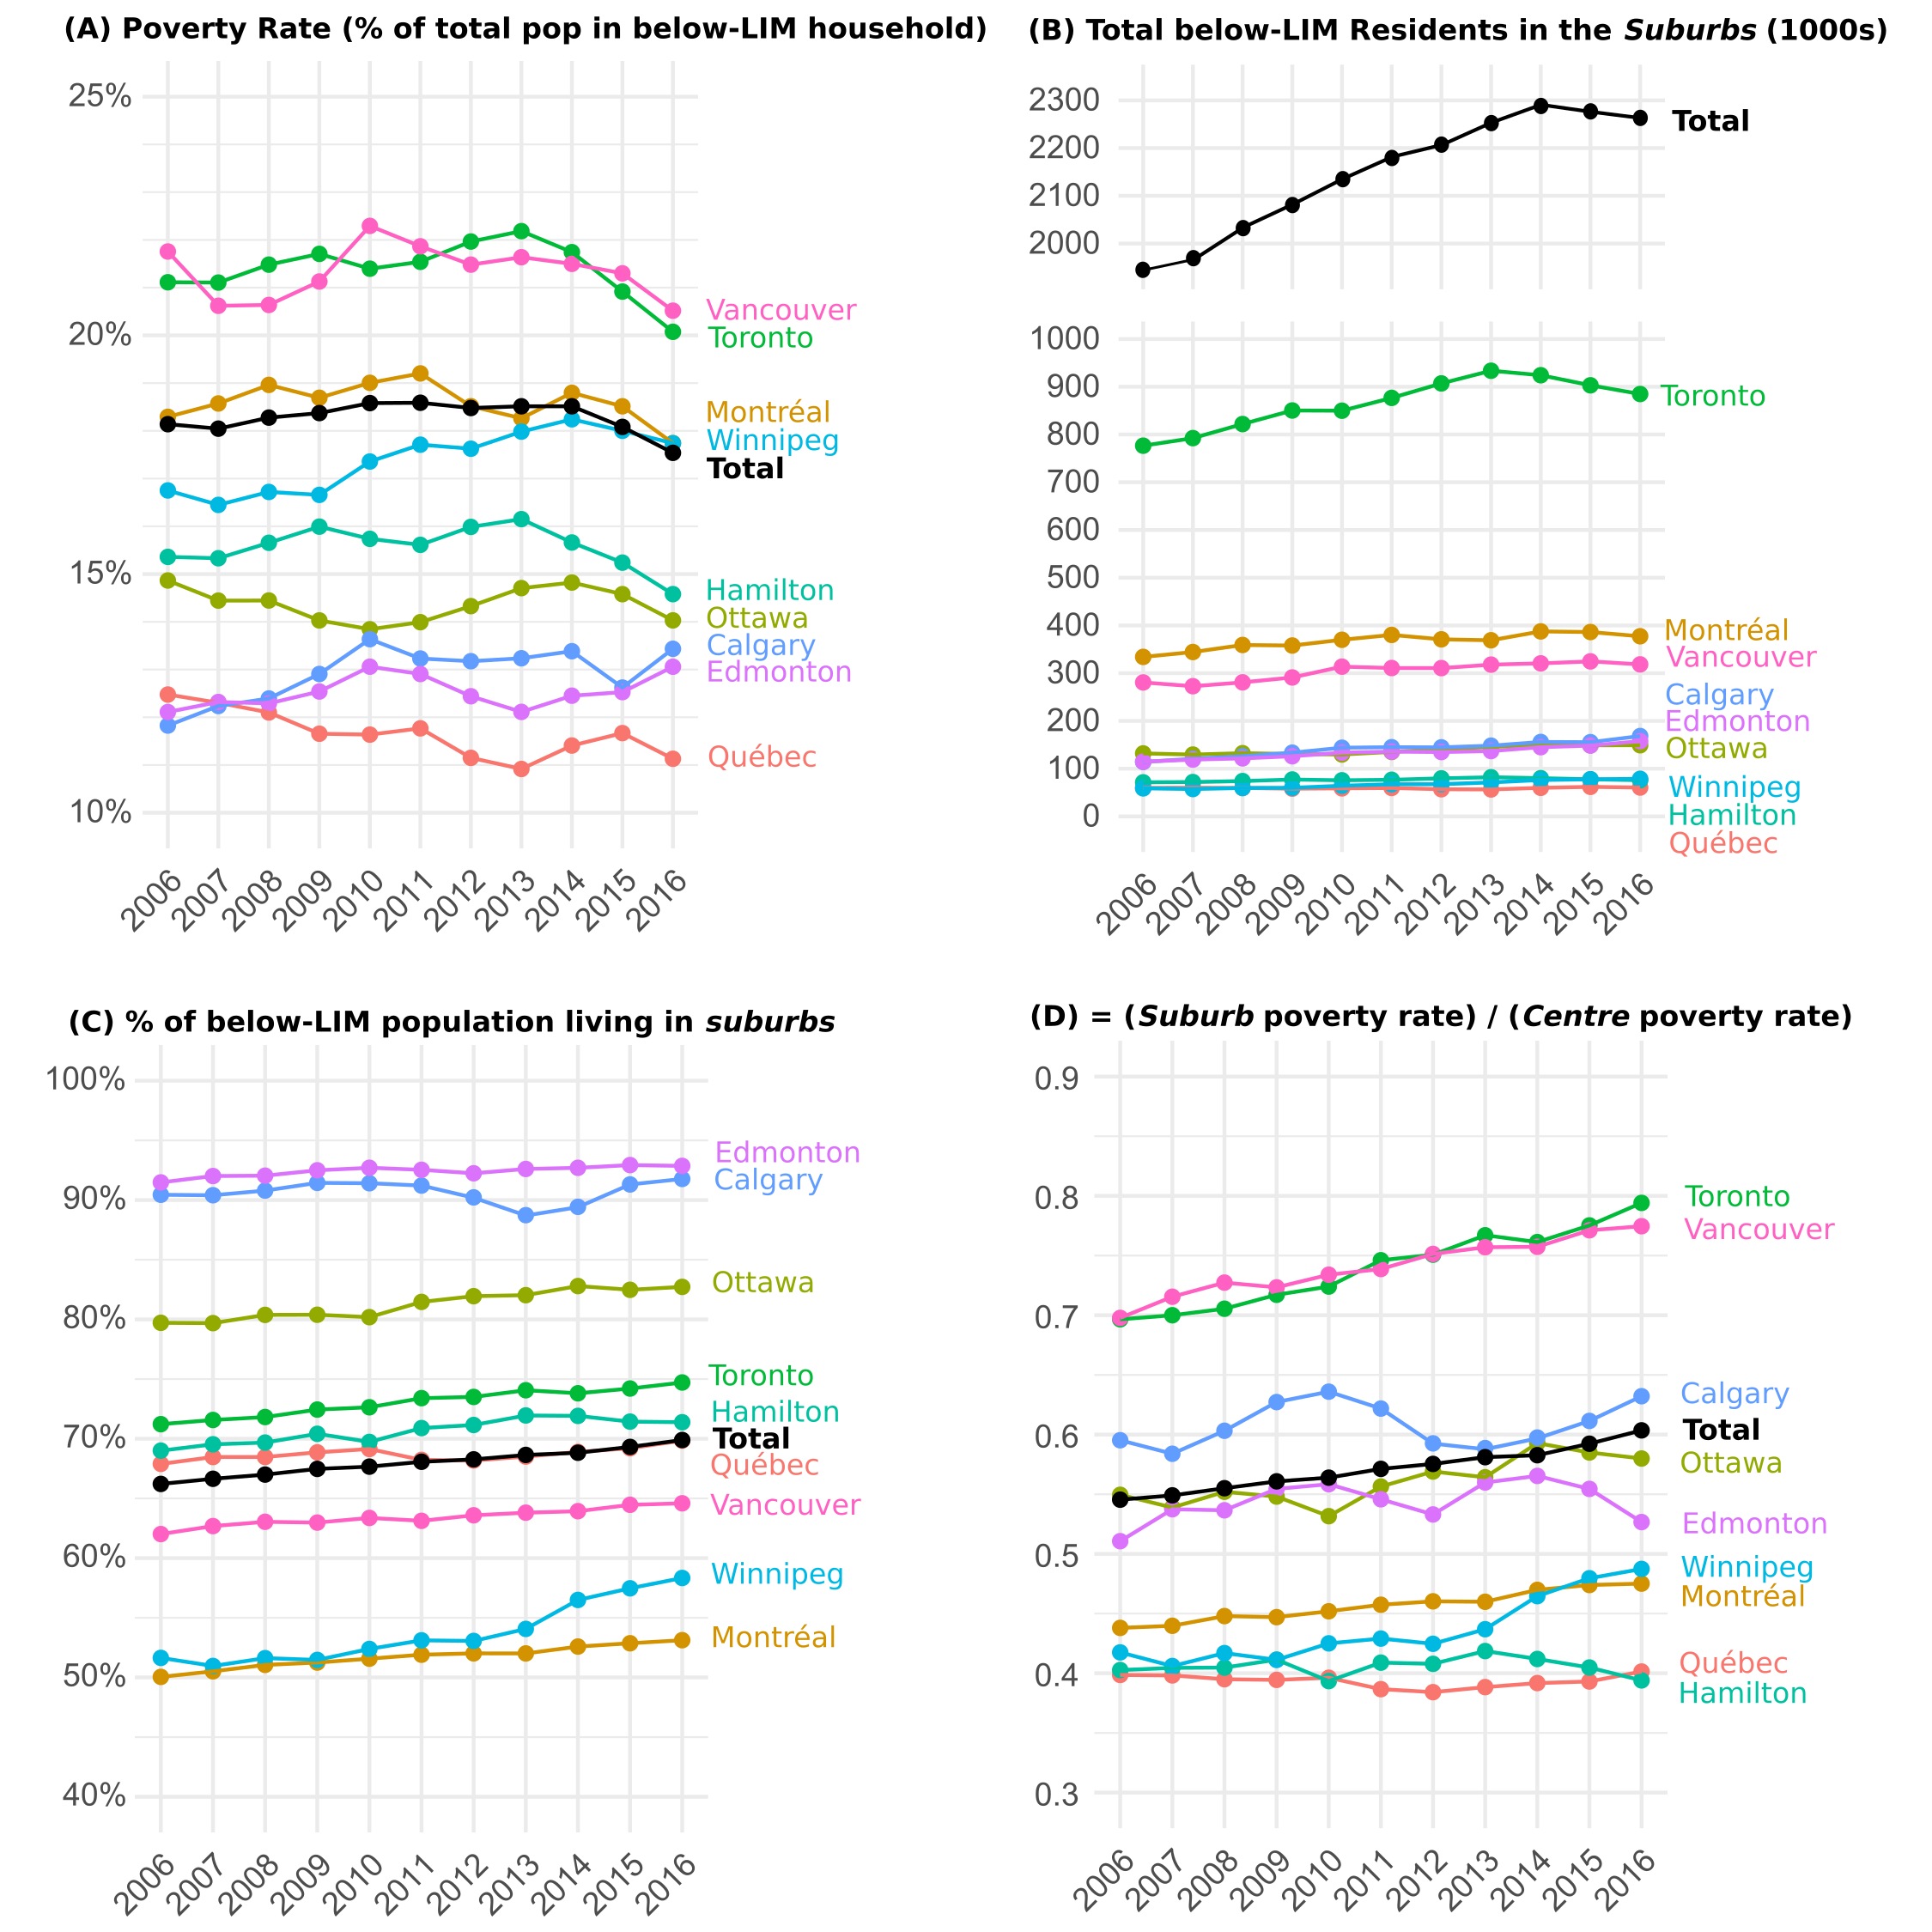
\includegraphics[width=6.5in]{figures/E_subpov4.png}
%	\end{center}
%	\caption{Plots tracking suburbanization of poverty in Canadian CMAs (2006 to 2016)}
%	\label{fig:subpov4}
%\end{figure*}





\begin{figure}[H]
	\centering
	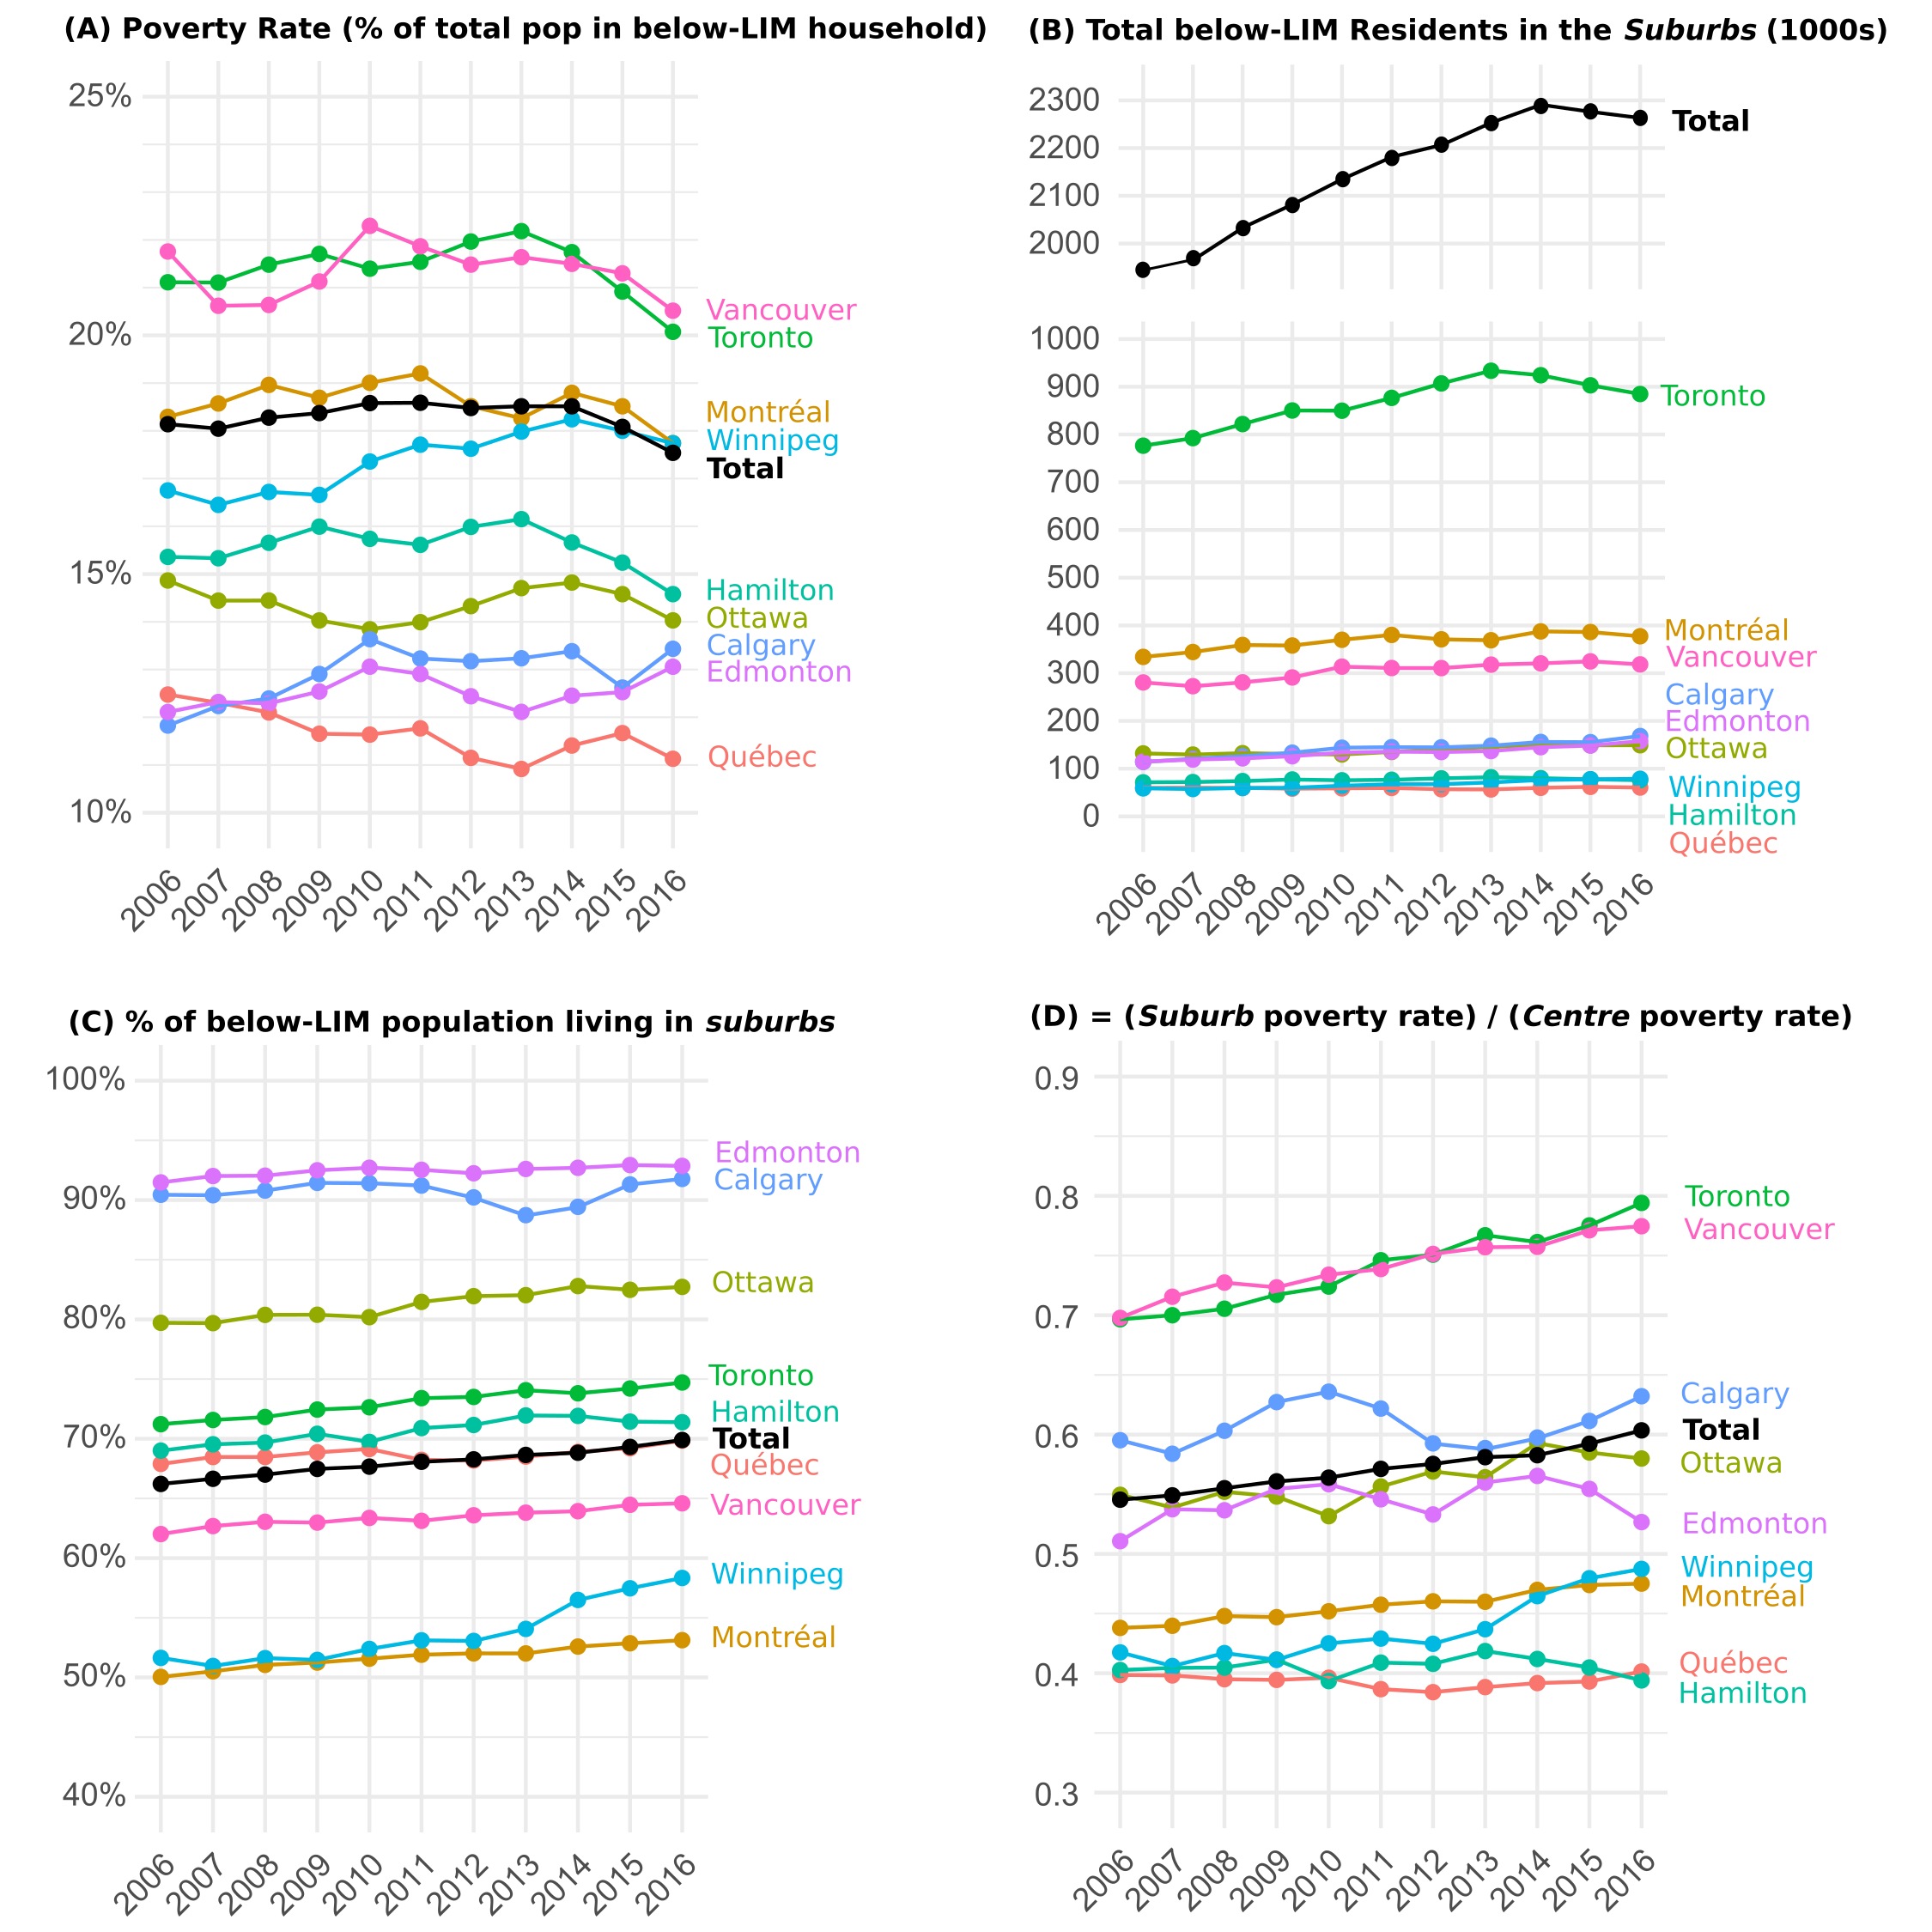
\includegraphics[width=6.5in]{figures/E_subpov4.png}
	\caption{Plots tracking suburbanization of poverty in Canadian CMAs (2006 to 2016)}
	\label{fig:subpov4}
\end{figure}


\subsection{Measuring Suburban Poverty}

In this section, we show how the prevalence of suburban poverty has changed over the study period (2006 to 2016) via a series of plots (Figure \ref{fig:subpov4}). First, for context, Figure \ref{fig:subpov4} (A) shows the overall poverty rate within each CMA based on the LIM. The larger cities (Vancouver, Toronto, and Montreal) have the greatest poverty rate, and overall, the poverty rate has declined over this ten year period, in particular form 2014 to 2016. Figure \ref{fig:subpov4} (B) shows the total count of residents under the poverty line living in neighbourhoods classified as \textit{suburbs}. We see that this is increasing up until 2014, when it drops slightly in concordance with an overall drop in the poverty rate. Figure \ref{fig:subpov4} (C) plots the percent of poverty in a CMA located in the \textit{suburbs}, showing increasing trends over time. However, the overall population living in the suburbs may also be increasing over this time period. Thus in Figure \ref{fig:subpov4} (D) we plot a ratio of the poverty rate in the \textit{suburbs} to the poverty rate in the \textit{centre}. Since this ratio is less than 1 in all cases, this indicates that the poverty rate remains greater in the centre than in the suburbs. However the gap between these two poverty rates is closing. Toronto and Vancouver are the two CMAs where this gap is narrowest and closing the quickest. These plots indicate that while the overall poverty rate in Canadian cities has declined slightly from 2006 to 2016, poverty in the suburbs has increased both in absolute and relative terms.






\subsection{Mobility Pathways to Suburban Poverty}

In our conceptual framework, we outlined three aggregate mobility pathways to suburban poverty: 1) centre-to-suburb, 2) immigration, and 3) staying in the suburbs. We now examine to what the extent of these pathways occur in Canadian CMAs. These pathways are summarized as proportions in Table \ref{table:p1} with current states, $j$, dichotomized by above-LIM and below-LIM households and by \textit{suburb} and \textit{centre}. Including these four states allows for showing how mobility pathways to suburban poverty (the rightmost column) differ from other states. We find that overall, for those in suburban poverty in Canadian CMAs, 88.5\% lived in the suburbs a year prior (12.7\% moved within the suburbs, 75.8\% stayed in the same postal code), 2.9\% moved from the \textit{centre}, and 6.6\% immigrated from elsewhere (4.6\% internationally). Overall, transitioning to suburban poverty on an annual basis is more due to staying or moving within the \textit{suburbs} compared to external immigration and moving from \textit{centre} neighbourhoods. Part of this finding is due to the suburbs being home to the majority of residents (77.8\%), but this doesn't tell the whole story. Importantly, looking at the low-income suburban residents who lived in the \textit{suburbs} a year prior, 21.5\% were not categorized as low-income in the previous year, meaning that becoming poor while staying in the suburbs encompass a greater percent of suburban poverty than moving in from elsewhere. Comparatively, those in poverty in the \textit{centre}, 15.4\% had dropped into poverty during the previous year. This difference indicates that residents are more likely to drop into poverty in suburban locations than in central, more accessible, neighbourhoods. This is likely partly explaining the trends shown in Figure \ref{fig:subpov4} (D) where the poverty rate in the \textit{suburbs} is increasing more than the poverty rate in the \textit{centre}. Similar to previous research in the United States \cite{delmelle_new_2020}, Table \ref{table:p1} also shows that residents in poverty are much more likely to have moved in the past year. Particularly notable is the extent of suburb-to-suburb mobility, 12.7\% for those in suburban poverty, compared to only 7.5\% for those not in poverty. 

\begin{table*}[h]
	\small
	\centering
	\begin{center}
		
		\caption{{Mobility pathways, $P(i|j)$, to different states, $j$, averaging across from 2006 to 2016 for residents in all 9 CMAs}}
		\label{table:p1}
		\begin{tabular}{llrrrr}
			\hline
			\multicolumn{2}{l}{}                        & \multicolumn{4}{c}{Current state, $j$}                  \\
			\multicolumn{2}{c}{}          & \multicolumn{2}{c}{Above poverty line} & \multicolumn{2}{c}{Below poverty line} \\
			Prior state, $i$                  & Prior poverty status      & \textit{Centre}       & \textit{Suburb}       & \textit{Centre}      & \textit{Suburb}    \\ \hline
			{International immigrant} &  & \textbf{0.6}          & \textbf{0.3}          & \textbf{5.2}         & \textbf{4.6}       \\ \arrayrulecolor{lightgray}\hline
			Internal migrant        & No              & 1.2          & 0.9          & 0.8         & 0.7       \\
			& Yes             & 0.2          & 0.1          & 1.2         & 1.3       \\ 
			\multicolumn{2}{l}{}                        & \textbf{1.4}          & \textbf{1.0}          & \textbf{2.0}         & \textbf{2.0}      \\ \arrayrulecolor{lightgray}\hline
			Moved from \textit{centre}         & No              & 5.8          & 1.2          & 2.3         & 0.7       \\
			& Yes             & 1.0          & 0.2          & 8.1         & 2.2       \\
			\multicolumn{2}{l}{}                        & \textbf{6.8}          & \textbf{1.4}         & \textbf{10.5}       & \textbf{2.9}      \\ \arrayrulecolor{lightgray}\hline
			Moved from \textit{suburbs}        & No              & 3.4          & 6.8          & 1.7         & 4.0       \\
			& Yes             & 0.5          & 0.8          & 3.8         & 8.7       \\
			\multicolumn{2}{l}{}                        & \textbf{3.9}          & \textbf{7.5}          & \textbf{5.4}         & \textbf{12.7}      \\ \arrayrulecolor{lightgray}\hline
			Stayed in same               & No              & 80.3         & 85.0         & 13.1        & 17.5      \\ 
			postal code & Yes             & 5.8          & 3.5          & 62.3        & 58.3      \\
			\multicolumn{2}{l}{}                        & \textbf{86.1}         & \textbf{88.5}         & \textbf{75.3}        & \textbf{75.8}      \\ \arrayrulecolor{lightgray}\hline
			\multicolumn{2}{l}{Births}                  &\textbf{ 1.2}         & \textbf{1.3}          & \textbf{1.6}         & \textbf{1.9}      \\ \arrayrulecolor{black}\hline
			\multicolumn{2}{l}{Total}                   & 100.0        & 100.0        & 100.0       & 100.0   \\ \arrayrulecolor{black}\hline
		\end{tabular}
	\end{center}
\end{table*}






\begin{figure}[H]
	\centering
	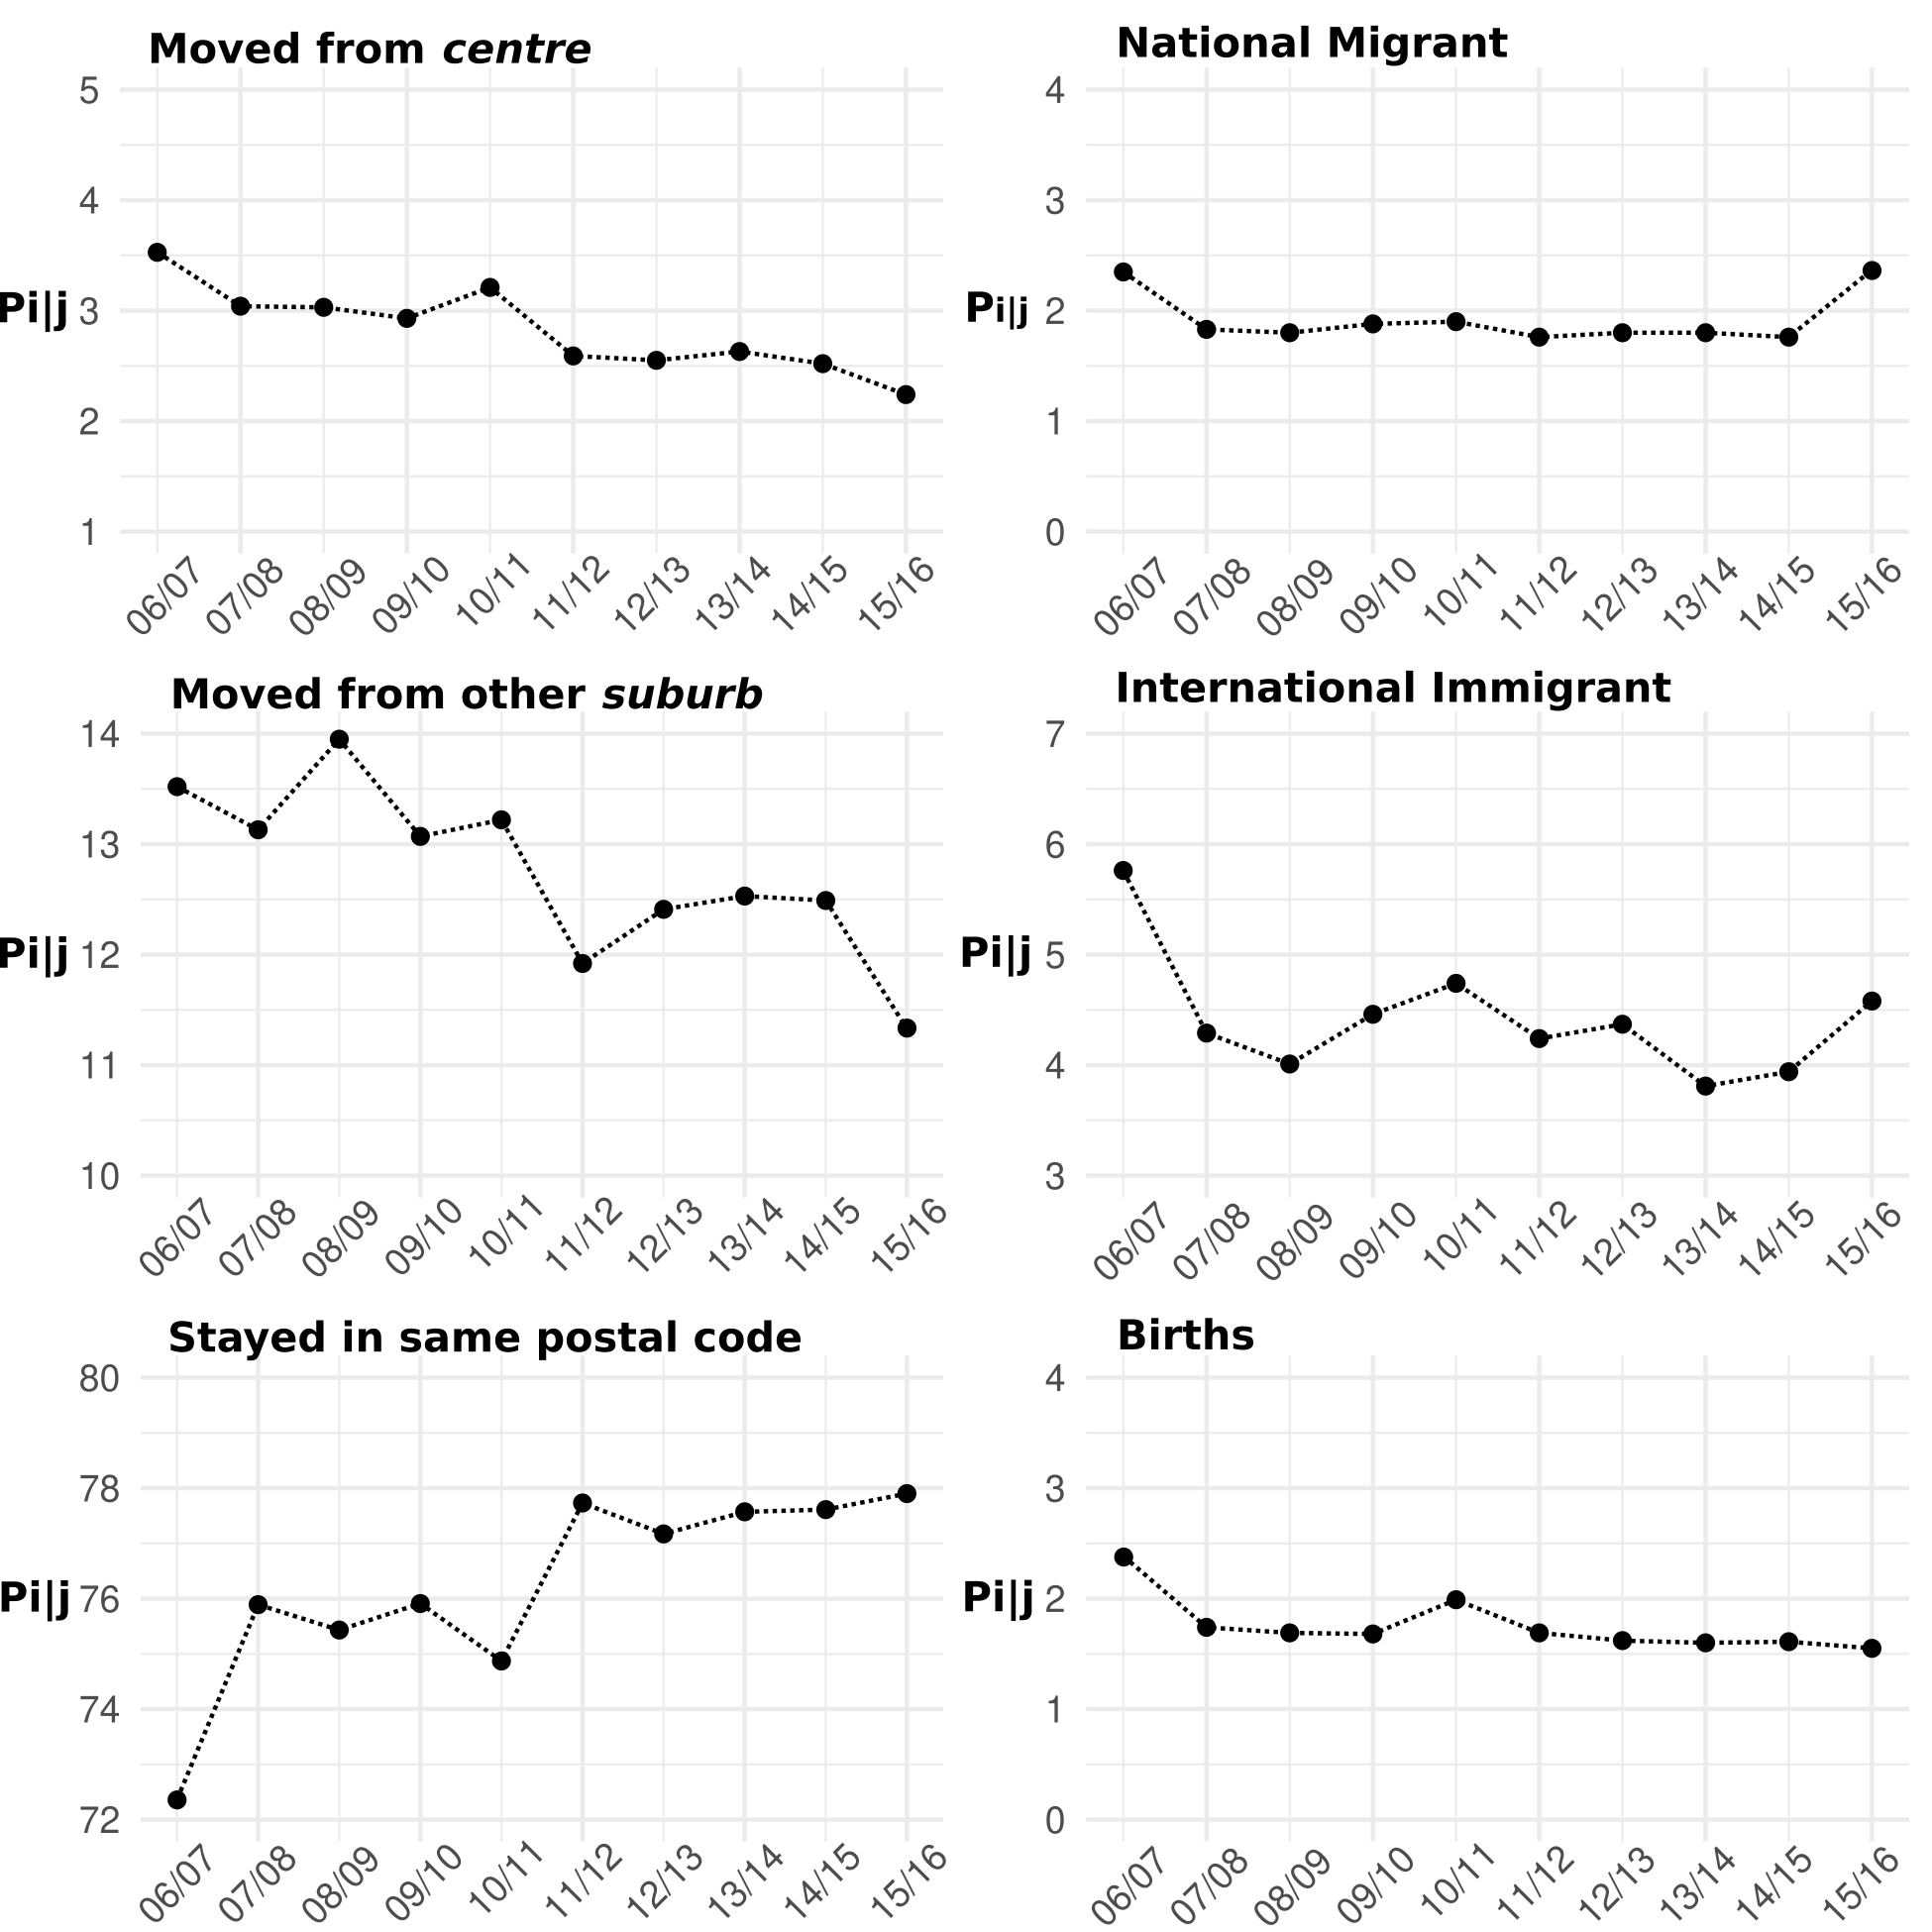
\includegraphics[width=4.9in]{figures/transitions_by_year.png}
	\caption{Mobility pathways, $P(i|j)$, to suburban poverty by year}
	\label{fig:tbyr}
\end{figure}


Figure \ref{fig:tbyr} shows how yearly transitions to suburban poverty have changed from 2006 to 2016. Overall, there has been a decline in the percentage of people in suburban poverty who moved from a different location within the region a year prior, both in terms of moving from another \textit{suburb} and moving from the \textit{centre}. This is offset by the proportion for not moving increasing over this time period. The percent of low-income immigrants from elsewhere in Canada and new births have remained relatively stable over time, while the proportion of international immigrants is a bit more sporadic.



We then turn our attention to differences in mobility transitions to suburban poverty by CMA (see Table \ref{table:pcma}). While the trends are relatively similar across all regions, there are some notable differences. The prairie cities of Edmonton, Calgary, and Winnipeg, show that not moving has lower proportions than the rest of Canada, while immigration, particularly international immigrants, account for a greater proportion of poverty in the suburbs in these cities. \textit{Suburb}-to-\textit{suburb} mobility is also greater in Edmonton and Calgary, mainly because the suburbs account for a relatively greater extent of the region than other cities (e.g. see Figure \ref{kcma}).  \textit{Centre}-to-\textit{suburb} residential mobility is greatest in Winnipeg, Vancouver, and Montreal indicating that gentrification-induced displacement may be greater in these three CMAs than in others. International immigration accounts for a greater proportion in Vancouver and Toronto than in other eastern cities. These two cities have high immigration rates over the study period, and have been described as having growing ethnic enclaves in suburban areas \cite{grant_changing_2020}. Of all nine CMAs, Hamilton has the greatest proportion of suburban poverty stemming from residents immigrating from elsewhere in Canada.






\begin{table}[h]
	\small
	\centering
	\caption{{Mobility pathways, $P(i|j)$, to suburban poverty by CMA (averaged from 2006 to 2016)}}
	\label{table:pcma}
	
	\makebox[\textwidth][c]{
		\begin{tabular}{ll p{1.2cm}p{1.2cm}p{0.9cm}p{1.1cm}p{1.1cm}p{1.0cm}p{0.9cm}p{1.0cm}p{1.0cm}}
			\hline
			&  &
			\multicolumn{9}{c}{CMA}                                                                                                                       \\
			Prior state, $i$                & Prior LIM & Vancouver     & Edmonton      & Calgary       & Winnipeg      & Hamilton      & Toronto       & Ottawa        & Montreal      & Quebec        \\ \hline
			International migrant &            & \textbf{4.6}  & \textbf{5.3}  & \textbf{6.5}  & \textbf{8.5}  & \textbf{2.6}  & \textbf{4.7}  & \textbf{3.4}  & \textbf{2.9}  & \textbf{2.5}  \\ \arrayrulecolor{lightgray}\hline
			Internal immigrant      & No         & 0.6           & 1.4           & 1.5           & 0.6           & 1.6           & 0.4           & 1.0           & 0.4           & 1.0           \\
			& Yes        & 1.2           & 2.7           & 2.6           & 1.0           & 3.0           & 1.0           & 1.9           & 0.7           & 1.5           \\
			\multicolumn{2}{l}{}                 & \textbf{1.8}  & \textbf{4.1}  & \textbf{4.1}  & \textbf{1.6}  & \textbf{4.6}  & \textbf{1.4}  & \textbf{2.9}  & \textbf{1.1}  & \textbf{2.5}  \\ \arrayrulecolor{lightgray}\hline
			Moved from \textit{centre}       & No         & 0.8           & 0.4           & 0.4           & 1.2           & 0.6           & 0.6           & 0.5           & 0.9           & 0.8           \\
			& Yes        & 2.5           & 0.9           & 0.8           & 3.8           & 1.9           & 1.8           & 1.8           & 3.0           & 2.2           \\
			\multicolumn{2}{l}{}                 & \textbf{3.3}  & \textbf{1.3}  & \textbf{1.2}  & \textbf{4.9}  & \textbf{2.6}  & \textbf{2.4}  & \textbf{2.3}  & \textbf{3.9}  & \textbf{2.9}  \\ \arrayrulecolor{lightgray}\hline
			Moved from \textit{suburbs}      & No         & 3.7           & 6.4           & 5.8           & 3.4           & 3.5           & 3.3           & 4.2           & 4.1           & 5.0           \\
			& Yes        & 8.7           & 10.6          & 9.5           & 7.5           & 6.9           & 8.6           & 9.3           & 7.8           & 7.3           \\
			\multicolumn{2}{l}{}                 & \textbf{12.4} & \textbf{17.0} & \textbf{15.3} & \textbf{10.9} & \textbf{10.4} & \textbf{11.9} & \textbf{13.5} & \textbf{11.9} & \textbf{12.2} \\ \arrayrulecolor{lightgray}\hline
			Stayed in same            & No         & 17.4          & 21.3          & 22.4          & 17.1          & 18.2          & 16.4          & 16.3          & 17.3          & 17.3          \\
			postal code & Yes        & 59.2          & 48.4          & 48.2          & 54.6          & 59.9          & 61.7          & 59.8          & 61.5          & 61.6          \\
			\multicolumn{2}{l}{}                 & \textbf{76.6} & \textbf{69.7} & \textbf{70.6} & \textbf{71.7} & \textbf{78.1} & \textbf{78.1} & \textbf{76.1} & \textbf{78.8} & \textbf{78.9} \\ \arrayrulecolor{lightgray}\hline
			\multicolumn{2}{l}{Births}           & \textbf{1.3}  & \textbf{2.6}  & \textbf{2.3}  & \textbf{2.4}  & \textbf{1.8}  & \textbf{1.6}  & \textbf{1.9}  & \textbf{1.4}  & \textbf{1.0}  \\ \arrayrulecolor{black}\hline
			\multicolumn{2}{l}{Total}            & 100.0         & 100.0         & 100.0         & 100.0         & 100.0         & 100.0         & 100.0         &  100.0         & 100.0 \\ \arrayrulecolor{black}\hline       
		\end{tabular}
	}
	
\end{table}



\vspace{5mm}

Lastly, we present probabilities of transitioning to states $j$ (such as suburban poverty), for different prior states $i$. This is presented in Table \ref{table:pji}. Noticeable from this table is that international immigrants, as well as internal migrants who were previously in poverty, have high propensities of moving to the suburbs and remaining under the poverty line. For international immigrants, this could partly be due to not having a full year of income (and thus being more likely to be classified as below the poverty line). Immigrating to the \textit{centre} also remains relatively high. We also find that those in poverty in the suburbs have a 24.9\% chance of moving out of poverty while staying in the suburbs. Included in Table \ref{table:pji} is the population size of $N_i$, averaged over the ten year period. Multiplying this by the percents can give is overall flows (the full flow matrix is also provided in the Appendix). This allows for showing the total flows in and out of suburban poverty. On average from 2006 to 2016, 471,000 residents living in the suburbs dropped into poverty per year, while 502,000 escaped poverty. While in the \textit{centre}, 157,000 dropped into poverty per year while staying in the \textit{centre}, while 181,000 escaped poverty. The relative difference in these ratios indicates that that poverty alleviation in-place is greater in the \textit{centre} than the \textit{suburbs} 



\begin{table}[h]
	\small
	\centering
	\caption{Propensities among different groups, $i$, of moving into suburban poverty}
	\label{table:pji}
	\begin{tabular}{llrrrrr}
		\hline 
		\multicolumn{2}{c}{}                        & \multicolumn{4}{c}{Current state, \textit{j}}   &               \\
		\multicolumn{2}{l}{Prior state, \textit{i}}          & \multicolumn{2}{c}{Non-LIM} & \multicolumn{2}{c}{LIM}  & \\ 
		Location                  & LIM status      & \textit{Centre}       & \textit{Suburb}       & \textit{Centre}      & \textit{Suburb}  & $\bar{N}_i$  \\ \hline
		International immigrant & & 8.1\%        & 15.7\%       & 26.4\%      & 49.8\%  &  196,626 \\ 
		\arrayrulecolor{lightgray}\hline
		Internal migrant        & No              & 20.9\%       & 64.6\%       & 5.0\%       & 9.5\% &  151,588   \\
		& Yes             & 7.8\%        & 22.1\%       & 21.1\%      & 49.0\%  &  58,251 \\
		\arrayrulecolor{lightgray}\hline
		\textit{Centre}                    & No              & 88.2\%       & 5.2\%        & 6.0\%       & 0.6\%  &  2,599,460  \\
		& Yes             & 18.8\%       & 2.0\%        & 74.3\%      & 4.8\%  & 961,042   \\
		\arrayrulecolor{lightgray}\hline
		\textit{Suburb}                    & No              & 0.8\%        & 94.8\%       & 0.2\%       & 4.2\%  & 11,213,758   \\
		& Yes             & 0.7\%        & 24.9\%       & 1.9\%       & 72.5\%   & 2,013,613 \\
		\arrayrulecolor{lightgray}\hline
		\multicolumn{2}{l}{Births}                  & 13.4\%       & 62.8\%       & 6.8\%       & 17.0\% & 229,551   \\ \arrayrulecolor{black}\hline
		Overall Totals            &                 & 15.3\%       & 66.4\%       & 5.8\%       & 12.5\%  & 17,423,889 \\ \hline
	\end{tabular}
\end{table}



\section{Conclusions}

Suburban poverty is an increasing phenomenon in Canadian cities. This is evident in our analysis of tax records (see Figure \ref{fig:subpov4}) as well as previous research using census and other survey data \cite{ades_are_2012,breau_pulling_2018,grant_changing_2020,allen_suburbanization_2021}.

In our research, we further set out to uncover the main residential mobility transitions to suburban poverty. We find that overall, transitioning to suburban poverty on an annual basis is much more a result from staying or becoming poor within the suburbs compared to immigration or due to moving (and potentially being displaced from) gentrifying neighbourhoods in the centre. On a year-by-year basis, of the low-income suburban residents who lived in the suburbs, 21.5\% dropped into poverty while staying in the suburbs on average, compared to only 2.9\% who moved from a central area or the 6.6\% who immigrated from elsewhere. We find that these trends are similar when comparing between regions and over our study period (2006 to 2016). Despite this finding, much of the discussion in Canada on suburbanization of poverty has been directly attributed to gentrification and displacement from less affordable central neighbourhoods \cite{grant_changing_2020}. This points to further consideration into the causes of dropping into poverty in the suburbs including (but not limited to), increasing rents in suburban apartments \cite{august_gentrification_2018}, automobile debt limiting spending in other areas \cite{walks_driving_2018}, or low transit accessibility impacting ability to travel to employment, education, or social services needed for poverty reduction \cite{allen_planning_2020} 

% Specifically, for those in suburban poverty in Canadian CMAs, 88.5\% lived in the suburbs a year prior (of which, 12.7\% moved residences within the suburbs and 75.8\% did not move), 2.9\% moved from a central neighbourhood, and 6.6\% immigrated from elsewhere (4.6\% internationally, 2.0\% from within in Canada). Moreover, of the low-income suburban residents who lived in the suburbs a year prior, 21.5\% were not classified as being in a low-income in the previous year. Thus becoming poor while staying in the suburbs encompasses a greater proportion of suburban poverty than immigration and \textit{centre}-to-\textit{suburb} mobility combined. 

Our results also provide pertinent information to aid preventative policy aimed at reducing suburban poverty in Canada. For one, knowledge that a substantial portion of suburban poverty stems from becoming poor in-place should expedite support for urban planning and policy to make suburbs more livable and accessible. In other words, policy for reducing suburban poverty should not parochially be focused on other pathways, such as limiting gentrification and displacement. While important to quell such displacement, our findings indicate that it is also imperative to make improvements to the suburbs, such as expanding community and social resources in the suburbs alongside more compact urban design, active travel infrastructure, and improved public transit in order to provide residents the ability to access amenities and opportunities (e.g. employment, education), as these would all be worthwhile strategies aimed at poverty alleviation in the suburbs. Our findings additionally show that international immigrants have a high propensity of settling in the suburbs and being below the poverty line. This points to policy aimed at providing incentives for more housing (e.g. as vouchers) for recent immigrants, particularly in more central locations. Overall, however, since our research was primarily descriptive and exploratory, future research should be designed to study the effectiveness of different strategies of reducing the propensity of dropping into poverty in the suburbs.

This is the first paper that we are aware of that develops a conceptual framework and empirically examines residential mobility pathways to suburban poverty. But given the exploratory nature of our analysis as well as use of a large-sample dataset, we had to make a few simplifications. As such, expanding upon these would also be important directions for future research. First, we used a single binary measure of low-income status (LIM) to classify whether a resident was in poverty in a given year. We used the LIM because it was pre-defined by Statistics Canada as well as used in other research projects \cite{picot_immigration_2014,allen_sizing_2019,brown_money_2019}. However, sensitivity analysis of results for different poverty measures, including those with multiple categories, would allow for more nuanced findings. Similarly, we generated a binary measure via a cluster analysis to describe whether or not a neighbourhood is suburban. This could be expanded to looking at multiple categories of urban form, in particular, specific types of suburban neighbourhoods. The $k$-means hierarchical clustering method we used could certainly be expanded to account for this. As well, other clustering methods could be tested to examine how and to what extent they would affect results.

Our analysis focused on year-to-year transitions from 2006 to 2016. So another important direction for future work would be to analyze individual pathways to suburban poverty prior to 2006 as well as analyze individuals over the course of multiple years. The latter could be conducted via sequence analysis methods to examine whether there are common life-course and residential mobility trajectories to suburban poverty. This could also be used to connect to longer-term neighborhood-level changes (e.g. to ask whether neighbourhoods with more concentrated poverty have a larger share of low-income people who dropped into poverty or who moved from elsewhere?). However, one drawback of using this tax record data is that it lacks contextual factors about why people move. Such factors are difficult to directly infer from tax records. Another direction for future work could be to link this data to possible push or pull factors that may disproportionately affect residential mobility of low-income residents. For example research analyzing out-mobility due to gentrification and new transit infrastructure has been conducted in the United States \cite{freeman_displacement_2005,delmelle_new_2020}, but not in Canada, and nowhere that we are aware of with the sample size of the LAD (20\% of the population). Continuing research in these directions would provide further knowledge regarding the individual pathways and neighbourhood dynamics that lead to suburbanization of poverty.






\section*{4.A \hspace{1mm} Appendix}
\addcontentsline{toc}{section}{4.A \hspace{1mm} Appendix}

\subsection*{4.A.1 \hspace{2mm} Measuring Transit Accessibility to Jobs}
\addcontentsline{toc}{subsection}{4.A.1 \hspace{2mm} Measuring Transit Accessibility to Jobs}


Transit accessibility measures were borrowed from the work by \citeA{allen_measure_2020}. These were calculated as follows.

\begin{equation}
A_{i,\lambda} = \frac{\bar A^o}{\bar A^c} \sum_{j = 1}^{J} \frac{ O_j f(t_{i,j,\lambda})}{L_{j}}
\end{equation}

$A_i$ is the accessibility measure from a zone $i$ for a transport mode $\lambda$. Where $O_j$ is the number of jobs at a zone $j$. $t_{i,j,\lambda}$ is the travel time from zone $i$ to $j$ by travel mode $\lambda$. $f(t_{i,j,\lambda})$ is a decay function weighting nearby locations more than those further away, computed as $f(t_{i,j,\lambda}) = e^{-0.023 t_{i,j,\lambda}}$. $L_j$ is a measure of access to the labour force from zone $j$. This accounts how in some regions places, there may be more jobs in proximity, but there may also be more people competing for those jobs (i.e. each job can only be filled by one worker). $L_j$ is computed as follows.

\begin{equation}
L_j = \sum_{\forall \lambda \in \Lambda} \sum_{i = 1}^{I} \frac{ \alpha_{i,\lambda} P_i f(t_{i,j,\lambda})}{A_{i,\lambda}}
\end{equation}



Where $P_i$ is the size of the labour force in zone $i$ and $\alpha_{i,\lambda}$ is the mode share for travel to work trips for mode, $\lambda$. $\Lambda$ is the overall set of travel modes, and the total mode share in each zone sums to 1, i.e. the above equation is subject to $\sum_{\forall \lambda \in \Lambda} { \alpha_{i,\lambda} = 1}$.

Since $L_j$ and $A_{i,\lambda}$ are dependent on each other, they were estimated iteratively. The fractional term in (1), $\frac{\bar A^o}{\bar A^c}$, standardizes after each iteration due to aggregate differences in the size of the labour force and total jobs in each region due to varying unemployment rates. $\bar A^o$ is the mean accessibility after the first iteration, and $\bar A^c$ is the mean accessibility after each iteration $c$.

Travel times, $t_{i,j,\lambda}$ were computed using OpenTripPlanner, incorporating walking networks from OpenStreetMap and GTFS data for transit schedules. Accessibility measures were computed for every minute during a morning commute period (7am to 9am), and then averaged, to account for fluctuating transit schedules. Population and employment data were based on the 2016 Canadian census. 


\subsection*{4.A.2 \hspace{2mm} Measuring Local Accessibility}
\addcontentsline{toc}{subsection}{4.A.2 \hspace{2mm} Measuring Local Accessibility}

Local accessibility measures were derived from the Proximity Measures Database (PMD) developed by \citeA{statistics_canada_proximity_2020}. Specifically, we generate an overall index based on proximity measures for the eight destinations noted in Table \ref{table:pmd} released at the dissemination block level. Each indicator in the PMB is released on a scale from 0 to 1, where a 0 is when there are no destinations within the network distance noted in Table \ref{table:pmd}, and a 1 is the highest value across all of Canada. All eight indicators were summed and then scaled into a standardized score prior to inputting into the cluster analysis.

\begin{table}[h]
	\small
	\centering
	\caption{{Destination types and network distances used to measure local accessibility}}
	\label{table:pmd}
	\begin{tabular}{lll}
		\hline
		\textbf{Destination}    & \textbf{Network Distance}   \\ \hline
		Grocery stores & 1km \\
		Health care & 3km \\
		Pharmacies & 1km \\
		Child care & 1.5km \\
		Primary education & 1.5km \\
		Secondary education & 1.5km \\
		Neighbourhood parks & 1km \\
		Libraries & 1.5km \\ 
		\hline
	\end{tabular}
\end{table}

\newpage



\subsection*{4.A.3 \hspace{2mm} Cluster Analysis Maps}
\addcontentsline{toc}{subsection}{4.A.3 \hspace{2mm} Cluster Analysis Maps}

Figures \ref{fig:mm1} and \ref{fig:mm2} show the spatial distribution of cluster analysis results for each CMA.


\begin{figure}[H]
	\centering
	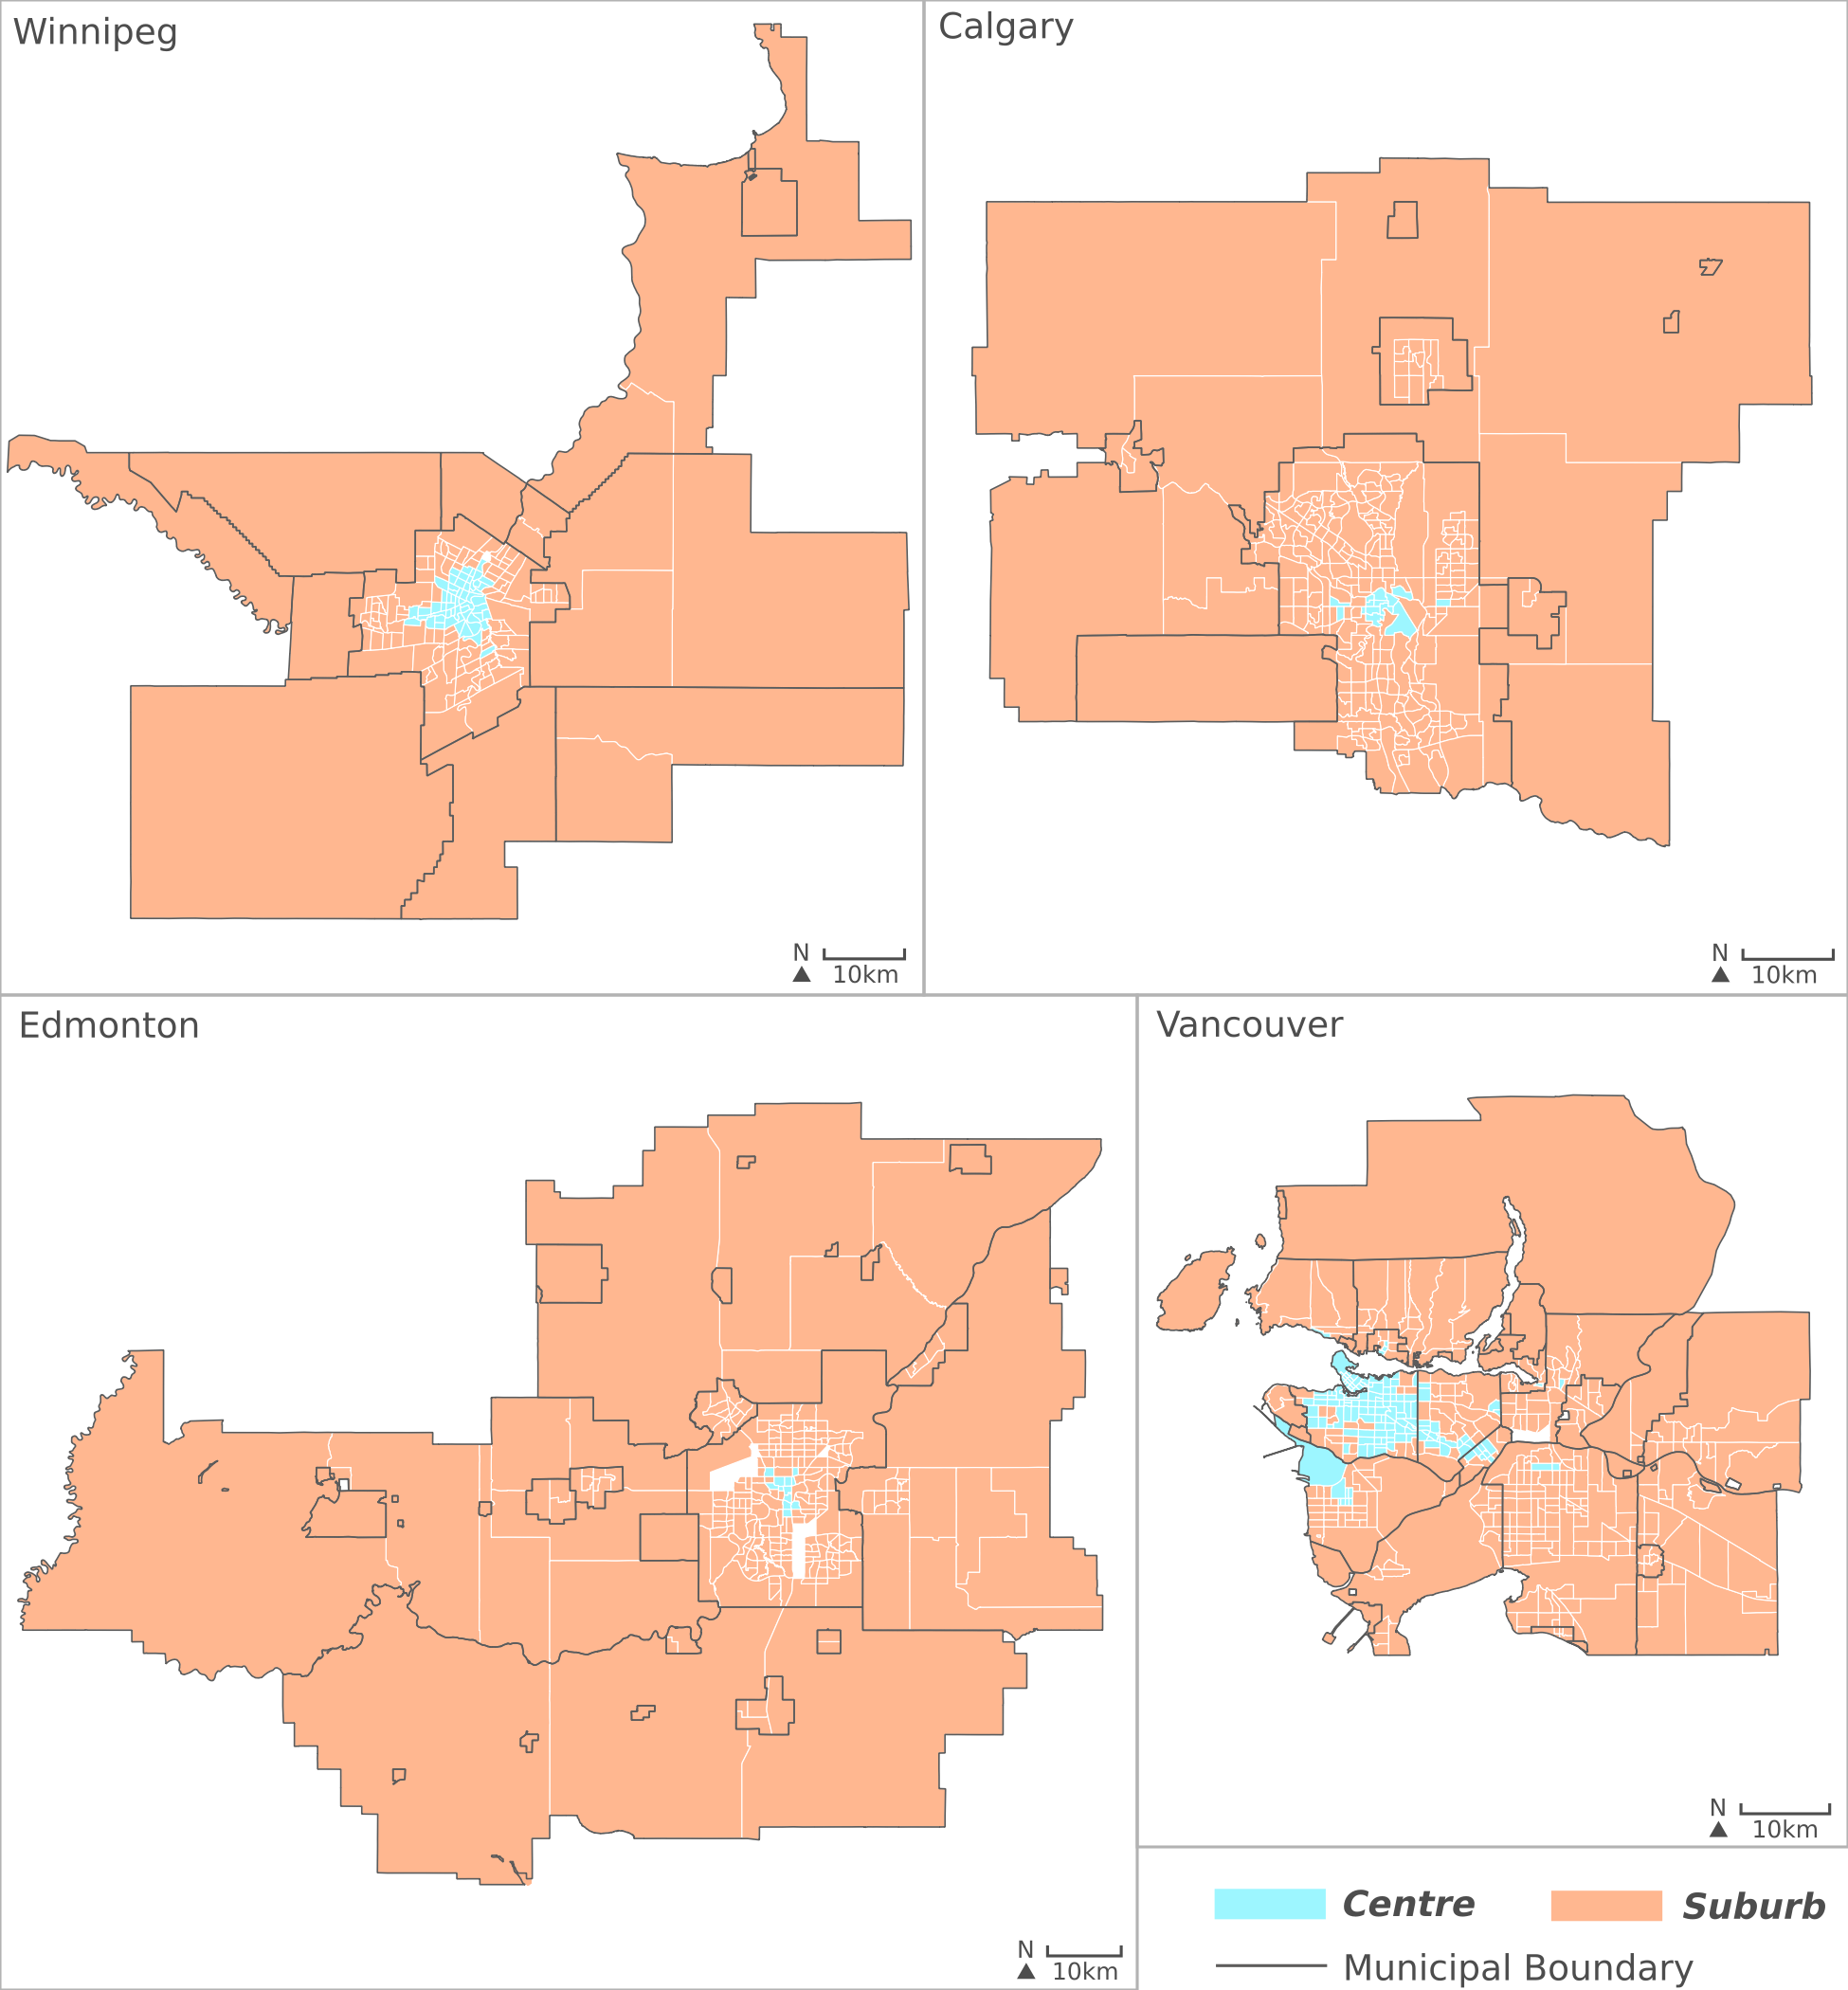
\includegraphics[width=6in]{figures/E_mini_2.png}
	\caption{Locations of \textit{centre} and \textit{suburb} clusters}
	\label{fig:mm1}
\end{figure}




\begin{figure}[H]
	\centering
	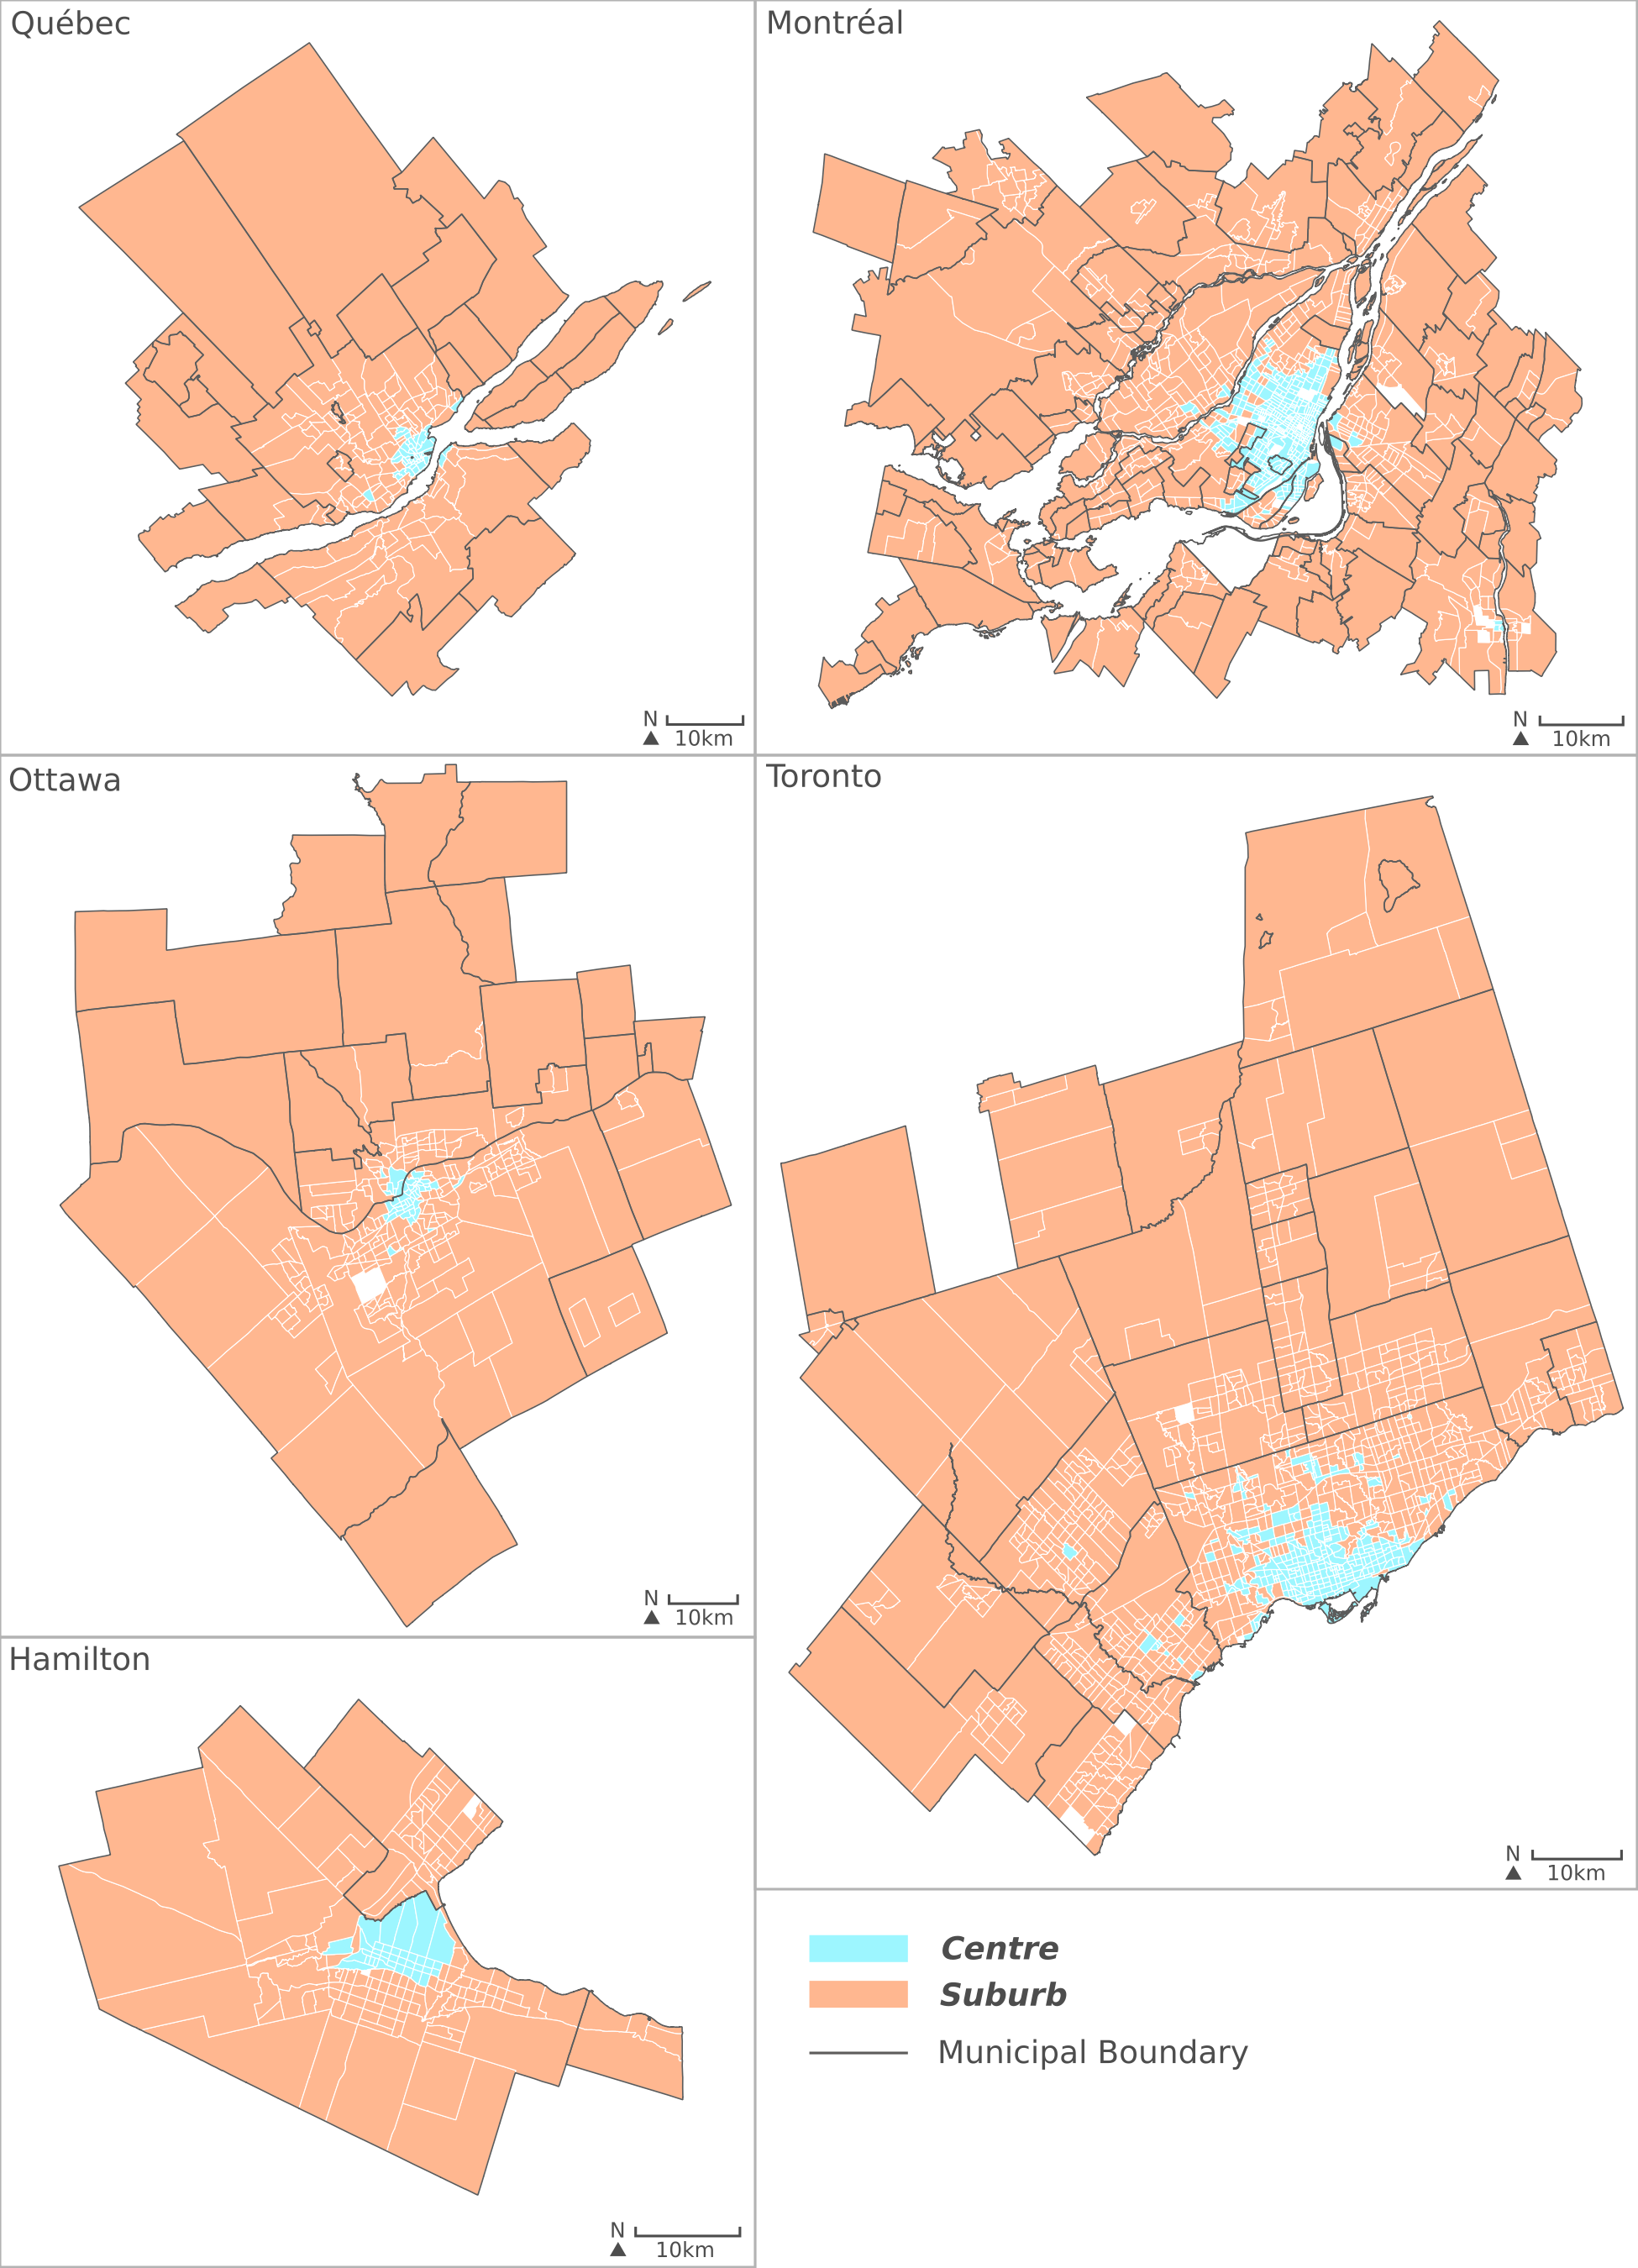
\includegraphics[width=6in]{figures/E_mini_1.png}
	\caption{Locations of \textit{centre} and \textit{suburb} clusters}
	\label{fig:mm2}
\end{figure}





\subsection*{4.A.4 \hspace{2mm} Population Flow Matrices}
\addcontentsline{toc}{subsection}{4.A.4 \hspace{2mm} Population Flow Matrices}




Table \ref{table:nij} displays average yearly population flows between different states $i$ and $j$. These values were used to generate the probabilities presented in Tables \ref{table:p1} and \ref{table:pji}.



\begin{table}[h]
	\small
	\centering
	\caption{Average yearly population flows, $\bar{N}_{i,j}$ between different states $i$ and $j$}
	\label{table:nij}
	\begin{tabular}{llrrrrr}
		\hline 
		\multicolumn{2}{c}{}                        & \multicolumn{4}{c}{Current state, \textit{j}}   &               \\
		\multicolumn{2}{l}{Prior state, \textit{i}}          & \multicolumn{2}{c}{Non-LIM} & \multicolumn{2}{c}{LIM}  & \\ 
		Location                  & LIM status      & \textit{Centre}       & \textit{Suburb}       & \textit{Centre}      & \textit{Suburb}  & Totals ($\bar{N}_i$)  \\ \hline
		
		
		International immigrant &  & 15,919    & 30,871     & 51,979    & 97,857    & 196,626    \\
		Internal migrant           & No           & 31,694    & 97,946     & 7,587     & 14,361    & 151,588    \\
		Internal migrant           & Yes          & 4,548     & 12,849     & 12,303    & 28,551    & 58,251     \\
		Centre                       & No           & 2,292,992 & 134,348    & 156,647   & 15,473    & 2,599,460  \\
		Centre                       & Yes          & 180,973   & 19,085     & 714,380   & 46,604    & 961,042    \\
		Suburb                       & No           & 91,585    & 10,633,223 & 16,914    & 472,036   & 11,213,758 \\
		Suburb                       & Yes          & 13,227    & 501,882    & 37,947    & 1,460,557 & 2,013,613  \\
		\multicolumn{2}{l}{Births}                  & 30,873    & 144,104    & 15,616    & 38,958    & 229,551    \\
		Totals ($\bar{N}_j$)                      &              & 2,661,811 & 11,574,308 & 1,013,373 & 2,174,397 & 17,423,889 \\ \hline
	\end{tabular}
\end{table}